\documentclass[11pt,a4paper]{article}

\usepackage[margin=2.35cm]{geometry}
\usepackage[T1]{fontenc}
\usepackage[utf8]{inputenc}
\usepackage{lmodern}
\usepackage{microtype}
\usepackage{amsmath,amssymb,mathtools,bm}
\usepackage{amsthm,empheq}
\usepackage{booktabs,tabularx,array,longtable}
\usepackage{graphicx}
\usepackage{placeins}
\usepackage{enumitem}
\usepackage[backend=biber,style=numeric,sorting=none,maxbibnames=99]{biblatex}
\addbibresource{references.bib}
\usepackage{hyperref}
\usepackage[nameinlink,noabbrev]{cleveref}
\usepackage{setspace}
\usepackage{xcolor}

\hypersetup{
  colorlinks=true,
  linkcolor=black,
  citecolor=black,
  urlcolor=blue,
  pdftitle={Schottky Response and Perplexity Tolerance in Locally Adaptive Clustering and Stochastic Neighbor Embedding},
  pdfauthor={Osvaldo L. Santos-Pereira}
}

\setlength{\parindent}{1.25em}
\setlength{\parskip}{0.18em}
\emergencystretch=2.5em
\onehalfspacing
\graphicspath{{figures/}}

\newcommand{\R}{\mathbb{R}}
\newcommand{\KL}{D_{\mathrm{KL}}}
\newcommand{\Var}{\operatorname{Var}}
\newcommand{\Perp}{\operatorname{Perp}}
\newcommand{\simplex}{\Delta}

\theoremstyle{definition}
\newtheorem{definition}{Definition}[section]
\crefname{definition}{definition}{definitions}
\Crefname{definition}{Definition}{Definitions}

\theoremstyle{plain}
\newtheorem{proposition}{Proposition}[section]
\newtheorem{corollary}[proposition]{Corollary}

% Discreet typographic separator marking the end of formal definitions.
\newcommand{\definitionseparator}{%
    \par\nobreak\vspace{0.15em}%
    \noindent\hfill
    \rule{0.19\linewidth}{0.30pt}%
    \hspace{0.65em}%
    {\scriptsize$\diamond$}%
    \hspace{0.65em}%
    \rule{0.19\linewidth}{0.30pt}%
    \hfill\mbox{}%
    \par\vspace{0.35em}%
}

\title{\textbf{Schottky Response and Perplexity Tolerance in Locally Adaptive Clustering and Stochastic Neighbor Embedding}}
\author{Osvaldo L. Santos-Pereira\\
\small Graduate Program in Multidisciplinary Applied Physics, Physics Institute,\\
\small Federal University of Rio de Janeiro, Rio de Janeiro, Brazil}
\date{}

\begin{document}

\maketitle

\begin{abstract}
The entropy-regularized feature weights of Locally Adaptive Clustering (LAC) define a finite feature ensemble whose response is controlled by gaps in the within-cluster dispersion spectrum. For an ideal two-level spectrum with $g_0$ low-dispersion and $g_1$ high-dispersion features, we derive the Schottky form $C=x^2u/(1+u)^2$, where $x=\Delta/h$ and $u=(g_1/g_0)e^{-x}$, and the peak condition $x=2(1+u)/(1-u)$. On the structured synthetic design, the resulting analytic peak predicts the true-partition response peak with at most 0.18\% relative error. In the initial $k$-means spectra, the gap-associated local peak remains within 11.51\% of the analytic scale, although within-band dispersion produces additional low-temperature maxima in two clusters. Across 30 realizations, a two-pass global response rule retains an adjusted Rand index (ARI) of $0.983\pm0.008$, close to the retrospective fixed-$h$ oracle at $0.988\pm0.006$, while independently selected cluster temperatures remain substantially worse. A separate matched-grid comparison evaluates response selection against silhouette and perturbation-stability selection, and controlled stress tests vary overlap, imbalance, dimensionality, and rotations that destroy axis-aligned feature relevance. For Stochastic Neighbor Embedding (SNE), the canonical response gives a first-order conversion between bandwidth and perplexity errors; direct perturbation tests on Wine at perplexities 5, 20, 30, and 50 quantify the accuracy of that linearization. The normalized-exponential identities are treated as classical prior structure; the new result is the spectral mechanism linking a LAC response peak to a feature-dispersion gap and its empirically testable failure conditions.
\end{abstract}

\noindent\textbf{Keywords:} statistical mechanics; Gibbs distribution; Shannon entropy; clustering; locally adaptive clustering; stochastic neighbor embedding; t-SNE; perplexity; dimensionality reduction; local metric learning.

\clearpage
\section*{Glossary}

\begin{longtable}{>{\raggedright\arraybackslash}p{0.22\textwidth} >{\raggedright\arraybackslash}p{0.72\textwidth}}
\toprule
\textbf{Term or symbol} & \textbf{Meaning}\\
\midrule
\endfirsthead
\toprule
\textbf{Term or symbol} & \textbf{Meaning}\\
\midrule
\endhead
LAC & Locally Adaptive Clustering.\\
SNE & Stochastic Neighbor Embedding.\\
t-SNE & t-distributed Stochastic Neighbor Embedding.\\
ARI & Adjusted Rand index.\\
KL divergence & Kullback--Leibler divergence.\\
DBSCAN & Density-Based Spatial Clustering of Applications with Noise.\\
LLE & Locally Linear Embedding.\\
UMAP & Uniform Manifold Approximation and Projection.\\
OLS & Ordinary least squares.\\
TLS & Total least squares.\\
WDBC & Breast Cancer Wisconsin Diagnostic dataset.\\
$X=(x_1,\ldots,x_n)$ & Dataset of $n$ observations $x_i\in\mathbb R^D$.\\
$\mathcal S$ & Generic finite state space; specialized to features $\mathbb F$ or candidate neighbors $\mathcal N_i$.\\
$\mathbb F$ & Finite LAC feature-state space.\\
$\mathcal N_i$ & Candidate-neighbor state space for SNE anchor $i$.\\
$p$ & Probability vector on a finite state space, with $p\in\Delta_{m-1}$.\\
$E_a$ & Dimensionless effective energy attached to state $a$.\\
$T$ & Positive canonical scale, termed effective temperature in the algorithmic analogy.\\
$S[p]$ & Shannon entropy of $p$ in nats.\\
$U[p]$ & Expected effective energy $\sum_a p_aE_a$.\\
$C(T)$ & Fixed-spectrum response $\partial U/\partial T=\operatorname{Var}(E)/T^2$; equal to dimensionless heat capacity in the canonical physical model.\\
Schottky response & Finite-system response peak generated by occupation transfer across a separated energy or dispersion gap.\\
$V_{\ell f}$ & Within-cluster dispersion of feature $f$ in LAC.\\
$w_{\ell f}$ & LAC feature-state probability for cluster $\ell$.\\
$h$ & LAC smoothing parameter and effective feature temperature.\\
$\sigma_i$ & Local Gaussian bandwidth for SNE anchor $i$.\\
$T_i^{(N)}=2\sigma_i^2$ & Local SNE neighbor temperature for anchor $i$.\\
$\Perp(P_i)$ & Perplexity of the local SNE neighbor distribution $P_i$.\\
$q_{ij}$ & Low-dimensional t-SNE pair probability.\\
\bottomrule
\end{longtable}

\clearpage
\tableofcontents
\clearpage


\section{Introduction}
\label{sec:introduction}

Clustering and dimensionality reduction are among the oldest unsupervised problems in multivariate analysis, but they answer different mathematical questions. A clustering procedure seeks a partition, or a related set-valued decomposition, that organizes observations according to a chosen notion of internal homogeneity and external separation. A dimensionality-reduction procedure instead seeks a mapping from a high-dimensional representation into a lower-dimensional space while preserving a specified geometric, statistical, or topological property. The two problems nevertheless share a central dependence on the geometry assigned to the observations. Distances, affinities, neighborhood scales, feature weights, and probability kernels determine what structure is visible to an algorithm. When the ambient dimension is large or the sampling density varies across the data space, a single global metric and a single global scale can be inadequate.

The historical development of clustering illustrates the progressive relaxation of restrictive geometric assumptions. The formulation of $k$-means by MacQueen, Ref.\,\cite{macqueen1967}, established a prototype of partition-based clustering in which observations are assigned to $K$ groups by minimizing within-cluster dispersion around representative means. Ward's hierarchical procedure, Ref.\,\cite{ward1963}, provided a complementary agglomerative construction based on controlling the increase of an objective function as groups are merged. Density-Based Spatial Clustering of Applications with Noise (DBSCAN), introduced by Ester et al., Ref.\,\cite{ester1996dbscan}, subsequently departed from convex or approximately spherical cluster assumptions by defining clusters through density connectivity and explicitly representing noise points. The spectral clustering construction of Ng, Jordan, and Weiss, Ref.\,\cite{ng2002spectral}, later recast partitioning in terms of eigenvectors of graph-derived matrices, allowing nonconvex structures to be separated after a nonlinear transformation of the similarity graph. The diversity of these approaches reflects a basic fact emphasized in broad reviews of cluster analysis Ref.\,\cite{jain1999review,jain2010clustering}: there is no unique mathematical definition of a cluster independent of the representation, similarity rule, and objective imposed on the data.

High-dimensional data created an additional difficulty because the relevance of coordinates can vary between groups. In a large ambient space, irrelevant or weakly informative variables may dominate Euclidean distances, while distinct clusters may occupy different coordinate subspaces. This problem motivated subspace and projected clustering. CLIQUE, Ref.\,\cite{agrawal1998clique}, searched automatically for dense units in axis-parallel subspaces, whereas PROCLUS, Ref.\,\cite{aggarwal1999proclus}, developed a projected-clustering formulation in which each cluster is associated with a subset of relevant dimensions. The survey of Kriegel, Kr\"oger, and Zimek, Ref.\,\cite{kriegel2009survey}, organized this literature into subspace, projected, pattern-based, and correlation-clustering families and emphasized that high-dimensional clustering requires explicit attention to local dimensional structure. Locally Adaptive Clustering (LAC), proposed by Domeniconi et al., Ref.\,\cite{domeniconi2007lac}, belongs naturally to this historical sequence: instead of selecting a single global subspace, it assigns cluster-dependent feature weights and thereby learns a local metric adapted to the dispersion structure of each group.

A particularly close precedent is the entropy-weighting $k$-means method of Jing, Ng, and Huang, Ref.\,\cite{jing2007entropy}, which also assigns cluster-dependent weights to dimensions and includes the entropy of those weights in the clustering objective. This prior work makes it essential to distinguish the present claim from entropy-weighted feature selection itself. The contribution developed below is instead the finite-spectrum response of the LAC weight distribution, the analytic two-level mechanism for its maximum, and tests of that response as a temperature-selection diagnostic.


Dimensionality reduction developed along a parallel line. Pearson's closest-fitting subspaces, Ref.\,\cite{pearson1901}, provided an early mathematical foundation for what later became principal component analysis, in which linear projection is determined by variance structure. Sammon's nonlinear mapping, Ref.\,\cite{sammon1969}, was designed to preserve pairwise dissimilarities with greater emphasis on smaller distances. Around 2000, manifold-learning methods shifted attention from global linear variance to local geometric relations. Isomap, introduced by Tenenbaum, de Silva, and Langford, Ref.\,\cite{tenenbaum2000isomap}, combined local metric information with graph geodesic distances to recover a global low-dimensional geometry, while Locally Linear Embedding (LLE), introduced by Roweis and Saul, Ref.\,\cite{roweis2000lle}, represented each observation by linear reconstruction weights computed from its neighbors and sought a lower-dimensional configuration preserving those weights. Laplacian Eigenmaps, formulated by Belkin and Niyogi, Ref.\,\cite{belkin2003laplacian}, provided a graph-spectral construction in which nearby observations are encouraged to remain close under an embedding derived from a graph Laplacian. These methods established locality as a central principle of nonlinear representation.

Stochastic Neighbor Embedding (SNE), introduced by Hinton and Roweis in 2002, Ref.\,\cite{hinton2002sne}, altered this perspective by representing neighborhoods probabilistically rather than only geometrically. For every observation, distances to the remaining observations are transformed into a conditional probability distribution. The embedding is then chosen so that low-dimensional conditional neighbor distributions approximate their high-dimensional counterparts according to the Kullback--Leibler divergence Ref.\,\cite{kullback1951}. t-distributed Stochastic Neighbor Embedding (t-SNE), introduced by van der Maaten and Hinton in 2008, Ref.\,\cite{vandermaaten2008tsne}, retained the probabilistic neighbor representation but symmetrized the high-dimensional affinities and replaced the Gaussian low-dimensional kernel by a Student kernel with one degree of freedom. This modification addressed the crowding problem and became influential in high-dimensional exploratory visualization. Later work reduced computational complexity through tree-based approximations Ref.\,\cite{vandermaaten2014}, clarified practical limitations and the dependence on hyperparameters Ref.\,\cite{wattenberg2016}, and developed related neighborhood-embedding methods such as Uniform Manifold Approximation and Projection (UMAP) Ref.\,\cite{mcinnes2018umap}. The subsequent use of t-SNE in high-dimensional biological data further motivated careful analysis of parameter choices and interpretation Ref.\,\cite{kobak2019}.

A second intellectual line relevant to the present work comes from information theory and statistical inference. Shannon's mathematical theory of communication Ref.\,\cite{shannon1948} introduced a quantitative measure of uncertainty for probability distributions and established entropy as a central information-theoretic functional. Kullback and Leibler Ref.\,\cite{kullback1951} subsequently formulated relative information between probability distributions, providing the divergence later adopted directly by SNE and t-SNE. Jaynes then connected these ideas to statistical mechanics in two companion papers, Refs.\,\cite{jaynes1957,jaynes1957ii}, by treating equilibrium distributions as solutions of constrained inference problems based on the maximization of Shannon entropy. In this formulation, the canonical exponential law is not introduced merely as a phenomenological probability rule: it follows from maximizing information entropy subject to normalization and expectation constraints. The resulting connection between Shannon's information measure, Gibbsian statistical mechanics, and constrained probabilistic inference supplies the conceptual basis for the entropy-optimization viewpoint adopted in this article.

The information-bottleneck construction of Tishby, Pereira, and Bialek, Ref.\,\cite{tishby1999ib}, provides another important variational precedent: it trades compression of one random variable against preservation of information about another. Its state variables and objective differ from LAC and SNE, but it reinforces the broader point that entropy-regularized learning objectives and temperature-like Lagrange multipliers predate the present analysis.


The historical strands represented by LAC and SNE/t-SNE are usually discussed separately. LAC adapts the metric by modifying the importance assigned to coordinates, whereas SNE adapts local probabilistic neighborhoods through point-dependent Gaussian bandwidths. Their mathematical structures, however, contain the same normalized exponential form. To state this observation precisely, consider a finite collection of states indexed by $a$ with dimensionless effective energies $E_a$. A normalized Gibbs distribution assigns larger probability to lower-energy states according to an exponential law. The canonical form that will organize the analysis is introduced here only as a preview; all symbols and assumptions are defined formally in Sec.\,\ref{sec:classical}:
\begin{equation}
    p_a
    =\frac{\exp(-E_a/T)}{\sum_b\exp(-E_b/T)},
    \label{eq:gibbs_intro}
\end{equation}
where $T>0$ is an effective temperature parameter. Eq.\,\eqref{eq:gibbs_intro} is introduced only as common notation. The existence of such a normalized exponential representation is classical and, as discussed in Sec.\,\ref{sec:related}, is not claimed as a contribution of this article.

This distinction determines the scope of the paper. The statistical-mechanical formulation of Gibbs Ref.\,\cite{gibbs1902}, the information entropy introduced by Shannon Ref.\,\cite{shannon1948}, and the maximum-entropy formulation developed by Jaynes Ref.\,\cite{jaynes1957} provide the classical relation between probability, entropy, constraints, and normalized exponential laws used below. The Kullback--Leibler divergence introduced by Kullback and Leibler Ref.\,\cite{kullback1951} supplies the information-theoretic discrepancy used by SNE and t-SNE. These established constructions are used here as a common baseline, not as results claimed by this article. The analysis instead asks what additional information is obtained when the underlying state variables are distinguished and when canonical response functions are evaluated on the LAC feature spectrum and the SNE neighbor spectrum. The logarithmic representation of a fixed positive t-SNE kernel is likewise treated as an algebraic identity; only its parameterized and response consequences are developed further. No appeal to R\'enyi or Tsallis entropy is required for this classical analysis.

The paper is organized as follows. Sec.\,\ref{sec:related} establishes the relevant priority and positions the contribution. Sec.\,\ref{sec:classical} defines the mathematical notation, information measures, the finite Gibbs variational problem, and canonical response functions. Sec.\,\ref{sec:lac} treats the LAC feature-weight subproblem with partition and centroids held fixed. Sec.\,\ref{sec:sne} treats SNE as a family of local neighbor-state ensembles. Sec.\,\ref{sec:tsne} analyzes t-SNE and energy-based fitting, while Sec.\,\ref{sec:unified} retains only the conditional generalized-Student observation needed for the state-space comparison. Sec.\,\ref{sec:unified} compares the distinct state spaces. Sec.\,\ref{sec:dual} defines the dual feature--neighbor construction and its Mahalanobis extension. Sec.\,\ref{sec:numerical} presents numerical response diagnostics, Sec.\,\ref{sec:limitations} states limitations and reproducibility conditions, and Sec.\,\ref{sec:conclusion} concludes.

\section{Related work and scope of the statistical-mechanical formulation}
\label{sec:related}

The statistical-mechanical terminology used in this paper has substantial prior art. It is therefore necessary to distinguish three claims that would otherwise be conflated: a generic Gibbs representation of positive probabilities, the established use of free-energy optimization in clustering, and the state-space comparison developed here. The first two are known results and are treated as such.

\subsection{Deterministic annealing and statistical mechanics of clustering}
\label{subsec:deterministic_annealing}

Rose, Gurewitz, and Fox, Ref.\,\cite{rose1990phase}, formulated fuzzy clustering by maximizing entropy at prescribed average distortion, identified the associated Lagrange multiplier with inverse temperature, and derived critical temperatures at which optimized cluster representations split. Rose, Ref.\,\cite{rose1998annealing}, subsequently developed deterministic annealing as a general framework for clustering, compression, classification, regression, and related optimization problems. Hofmann and Buhmann, Ref.\,\cite{hofmann1997pairwise}, extended the same free-energy logic to pairwise data clustering. Neal and Hinton, Ref.\,\cite{neal1998em}, provided a closely related variational precedent for alternating statistical algorithms by expressing expectation--maximization as coordinate optimization of a free-energy-like functional over model parameters and distributions of latent variables. That precedent is methodologically relevant to LAC because LAC likewise alternates between assignments, representatives, and feature weights, even though the state variable studied here is different. These works predate LAC and establish priority for the use of energy, entropy, free energy, temperature, and phase-transition language in clustering.

A distinct statistical-physics route was developed by Blatt, Wiseman, and Domany, Ref.\,\cite{blatt1996spc}, who mapped observations to interacting Potts spins and identified clusters through spin correlations in a superparamagnetic regime. Their later analysis, Ref.\,\cite{wiseman1998spc}, examined the thermodynamic behavior of the inhomogeneous Potts construction in greater detail. This literature is directly relevant to any proposal that uses susceptibility- or heat-capacity-like extrema to select clustering scales: there the thermodynamic observables arise from an interacting spin model on a neighborhood graph, whereas the response studied below is computed from a finite spectrum of feature dispersions in the LAC weight subproblem. The distinction in state variable and interaction structure is therefore essential; the use of thermodynamic response as a clustering diagnostic is not new in itself.

The state variable in deterministic annealing is principally an assignment or codevector state: probability is distributed over possible cluster associations for an observation. The LAC subproblem studied in Sec.\,\ref{sec:lac} is different. Once the hard partition and centroids are fixed, the probability vector is indexed by input features. Thus the present article does not introduce a statistical-mechanical formulation of clustering. Its narrower structural observation is that the same classical variational principle acts on a distinct finite state space---feature labels---and can then be compared with the neighbor-state space of SNE.

\subsection{Energy-based models and neighbor embeddings}
\label{subsec:ebm_related}

Normalized exponential probabilities also have a long history outside statistical mechanics. Bridle, Ref.\,\cite{bridle1990softmax}, introduced the normalized exponential or softmax transformation for probabilistic interpretation of neural-classifier outputs and explicitly related it to Boltzmann normalization. Energy-based learning later provided a broader framework in which scalar energies are converted into normalized probabilities through a Gibbs distribution. LeCun et al., Ref.\,\cite{lecun2006ebm}, explicitly note that sufficiently broad probability families can be represented by suitable redefinitions of the energy. Consequently, for a strictly positive kernel $k(r)$, the identity $k(r)=\exp\left[-(-\ln\left(k(r)\right))\right]$ is mathematically exact but does not by itself impose a restriction or generate a prediction. The logarithmic-energy representation of the t-SNE kernel must therefore be treated as an algebraic reparameterization unless additional structure is extracted from it.

That additional structure has been studied in the neighbor-embedding literature. Carreira-Perpi\~n\'an, Ref.\,\cite{carreira2010elastic}, decomposed SNE into attractive and repulsive contributions and developed Elastic Embedding from this viewpoint. B\"ohm, Berens, and Kobak, Ref.\,\cite{bohm2022spectrum}, organized neighbor-embedding objectives along an attraction--repulsion spectrum. Damrich et al., Ref.\,\cite{damrich2023contrastive}, connected t-SNE and UMAP through contrastive-learning objectives and characterized the distortion induced by negative sampling. Theoretical analyses of t-SNE include Arora, Hu, and Kothari, Ref.\,\cite{arora2018analysis}, and the early-exaggeration regime studied by Linderman and Steinerberger, Ref.\,\cite{linderman2019provably}. The pointwise bandwidth construction itself has been studied as an entropic-affinity problem by Vladymyrov and Carreira-Perpi\~n\'an, Ref.\,\cite{vladymyrov2013entropic}, who analyze the locally adaptive widths defined by a prescribed perplexity; more recent work by Van Assel et al., Ref.\,\cite{vanassel2023snekhorn}, likewise emphasizes that such affinities adapt to heterogeneous sampling densities by enforcing row-wise entropy. Vladymyrov and Carreira-Perpi\~n\'an also exploit derivatives of the entropy with respect to the affinity scale as an internal numerical device for solving the perplexity constraint. The present use is narrower and operationally different: the same derivative is reported as an anchor-wise response statistic and converted into an explicit tolerance on the bandwidth search. The generalized heavy-tailed t-SNE family of Kobak et al., Ref.\,\cite{kobak2020heavy}, will be used in Sec.\,\ref{sec:tsne} because its degrees-of-freedom parameter provides a nontrivial parametric structure beyond the tautological map $E=-\ln\left(k\right)$.

\subsection{Contribution and limits of the present work}
\label{subsec:contribution_scope}

The contribution is therefore not to establish that LAC or SNE can be written with Gibbs factors. The paper makes three empirical or operational claims and one prospective construction. First, the fixed-spectrum LAC response is tested as a temperature-selection diagnostic across 30 realizations of one structurally heterogeneous synthetic design. Two global rules are distinguished: an adaptive rule that recomputes $h$ during the alternating scheme and a two-pass rule that estimates $h$ once and then freezes it. Their convergence behavior, near-optimal ARI plateau, sensitivity to feature standardization, and performance on three real clustering benchmarks are reported explicitly. Second, the SNE response is used to convert a target perplexity tolerance into a local first-order bandwidth tolerance and is evaluated together with controlled density-scaling and errors-in-variables experiments. Third, deterministic annealing is run on the same synthetic geometry to demonstrate an assignment bifurcation absent from a fixed feature spectrum. The generalized Student analysis is retained only as a conditional observation after the quadratic pair-energy coordinate has been fixed. Finally, a dual feature--neighbor ensemble is stated as a prospective synthesis; its convergence and predictive performance are not claimed here.

\section{Mathematical preliminaries and the classical canonical ensemble}
\label{sec:classical}

The comparison between clustering, neighbor embedding, and statistical mechanics requires a precise common notation. This section therefore introduces the data space, probability distributions, information measures, and canonical variational problem before any algorithm-specific identification is made. The definitions are standard, but stating them explicitly is important because the same symbols will later acquire algorithmic interpretations as feature weights, neighbor probabilities, effective energies, and effective temperatures.

\subsection{Data, partitions, probability distributions, and information measures}
\label{subsec:notation}


\begin{definition}[Dataset]
\label{def:dataset}
Let $n,D\in\mathbb{N}$, with $n\ge1$ and $D\ge1$, and define the observation index set $I_n=\{1,\ldots,n\}$ and the feature index set $I_D=\{1,\ldots,D\}$. A finite real-valued dataset is an indexed family of $n$ observations in the $D$-dimensional Euclidean feature space $\R^D$. This representation is standard in clustering and pattern-analysis formulations, in which observations are treated as feature vectors before a similarity or dissimilarity rule is imposed Ref.\,\cite{jain1999review}. We write the dataset as
\begin{equation}
    X=(x_1,\ldots,x_n)\in(\R^D)^n.
    \label{eq:dataset}
\end{equation}
Here $X$ is an indexed family rather than a set in the strict set-theoretic sense; consequently, two distinct observation indices may correspond to identical feature vectors without being identified.

For each $i\in I_n$, the observation $x_i$ is the column vector
\begin{equation}
    x_i=(x_{i1},\ldots,x_{iD})^{\mathsf T}\in\R^D,
    \label{eq:observation_vector}
\end{equation}
where $x_{if}\in\R$ denotes the measured value of feature $f\in I_D$ for observation $i$. Thus the first index identifies an observation and the second identifies a feature.

Unless another metric is introduced explicitly, distances in the ambient space are Euclidean. For observations $x_i$ and $x_j$, the squared Euclidean distance is
\begin{equation}
    \|x_i-x_j\|_2^2
    =\sum_{f=1}^{D}(x_{if}-x_{jf})^2.
    \label{eq:euclidean_distance}
\end{equation}
Eq.\,\eqref{eq:euclidean_distance} separates the contribution of each measured feature to the total squared separation and will later be modified by LAC through feature-dependent weights.
\end{definition}
\definitionseparator

The notation in Definition~\ref{def:dataset} can be read directly as a rectangular data table. Each row corresponds to one indexed observation $x_i$, each column corresponds to one feature, and the entry in row $i$ and feature column $f$ is the scalar $x_{if}$. Tab.\,\ref{tab:dataset_notation} provides a symbolic example without introducing any additional assumptions about the numerical values.

\begin{table}[htbp]
\centering
\begingroup
\renewcommand{\arraystretch}{1.30}
\caption{Symbolic representation of the dataset $X$ defined in Eq.\,\eqref{eq:dataset} and Eq.\,\eqref{eq:observation_vector}. Rows represent observations and columns represent measured features.}
\label{tab:dataset_notation}
\begin{tabular}{c c c c c}
\toprule
Observation & Feature $1$ & Feature $2$ & $\cdots$ & Feature $D$\\
\midrule
$x_1$ & $x_{11}$ & $x_{12}$ & $\cdots$ & $x_{1D}$\\
$x_2$ & $x_{21}$ & $x_{22}$ & $\cdots$ & $x_{2D}$\\
$\vdots$ & $\vdots$ & $\vdots$ & $\ddots$ & $\vdots$\\
$x_n$ & $x_{n1}$ & $x_{n2}$ & $\cdots$ & $x_{nD}$\\
\bottomrule
\end{tabular}
\endgroup
\end{table}

\begin{definition}[Cluster and hard clustering]
\label{def:hard_clustering}
For the dataset in Definition~\ref{def:dataset}, a \emph{cluster} is represented by a nonempty subset of observation indices. A \emph{hard clustering} into $K\in\mathbb{N}$ clusters is a partition of $I_n$ into $K$ nonempty blocks. This partition-based representation is standard in classical cluster analysis Ref.\,\cite{jain1999review,jain2010clustering}. Formally, a family $\{C_1,\ldots,C_K\}$ defines a hard clustering when the following three conditions hold:
\begin{subequations}
\label{eq:hard_clustering_conditions}
\begin{empheq}[left=\empheqlbrace]{align}
    C_\ell &\subseteq I_n,\qquad C_\ell\neq\varnothing,\qquad \ell=1,\ldots,K,
    \label{eq:cluster_nonempty}\\
    C_\ell\cap C_r &=\varnothing,\qquad \ell\neq r,
    \label{eq:cluster_disjoint}\\
    \bigcup_{\ell=1}^{K}C_\ell &= I_n.
    \label{eq:cluster_exhaustive}
\end{empheq}
\end{subequations}
Eq.\,\eqref{eq:cluster_nonempty} states that each cluster $C_\ell$ is a subset of the observation index set $I_n$ and is nonempty. The associated observations are therefore the subfamily $\{x_i:i\in C_\ell\}$ of the dataset. The nonemptiness requirement excludes vacuous blocks and ensures that cluster-dependent quantities, such as centroids and within-cluster dispersions, are defined whenever their usual finite-sample formulas are employed.

Eq.\,\eqref{eq:cluster_disjoint} imposes pairwise disjointness. For any two distinct cluster labels $\ell$ and $r$, the intersection $C_\ell\cap C_r$ is empty. This condition gives the assignment its \emph{hard} character: no observation index can belong simultaneously to two distinct clusters.

Eq.\,\eqref{eq:cluster_exhaustive} imposes exhaustivity. The union of all $K$ clusters equals the full observation index set $I_n$, so every observation index is assigned to at least one cluster. Together with Eq.\,\eqref{eq:cluster_disjoint}, this implies that every observation index belongs to exactly one cluster. Consequently, Eqs.\,\eqref{eq:cluster_nonempty}--\eqref{eq:cluster_exhaustive} define a partition of $I_n$ into $K$ nonempty blocks and distinguish hard clustering from overlapping, fuzzy, or possibilistic formulations.
\end{definition}
\definitionseparator

\begin{definition}[Finite state space, probability mass function, probability vector, and probability simplex]
\label{def:finite_probability_space}
Let
\begin{equation}
    \mathcal{X}_m
    :=\{\xi_1,\ldots,\xi_m\},
    \qquad
    |\mathcal{X}_m|=m\ge2,
    \label{eq:finite_state_space}
\end{equation}
be a finite state space, also called a finite alphabet in information theory. A probability mass function on \(\mathcal{X}_m\) is a mapping
\begin{equation}
    p:\mathcal{X}_m\longrightarrow[0,1],
    \qquad
    \xi_a\longmapsto p(\xi_a)=:p_a,
    \label{eq:pmf_mapping}
\end{equation}
such that the probability assigned to each state is nonnegative and the total probability equals one. The ordered vector \(p=(p_1,\ldots,p_m)\in\mathbb{R}^m\) is the probability vector associated with the mass function. The set of all probability vectors on \(\mathcal{X}_m\) is defined formally as the \((m-1)\)-dimensional probability simplex
\begin{equation}
    \Delta_{m-1}
    :=\left\{
        p=(p_1,\ldots,p_m)\in\mathbb{R}^m:
        p_a\ge0\ \text{for all }a,
        \ \sum_{a=1}^{m}p_a=1
    \right\}.
    \label{eq:probability_simplex_set}
\end{equation}
This set-comprehension definition is the standard finite probability simplex used in convex analysis and information theory, Ref.\,\cite{boyd2004,cover2006}. Equivalently, membership of \(p\) in \(\Delta_{m-1}\) may be displayed through the following state-probability and normalization relations:
\begin{subequations}
\label{eq:probability_simplex}
\begin{empheq}[left=\empheqlbrace]{align}
    p_a &= p(\xi_a),
    \qquad a=1,\ldots,m,
    \label{eq:state_probability}\\
    p_a &\ge0,
    \qquad a=1,\ldots,m,
    \label{eq:probability_nonnegative}\\
    \sum_{a=1}^{m}p_a &=1.
    \label{eq:probability_normalization}
\end{empheq}
\end{subequations}
Eq.\,\eqref{eq:state_probability} identifies the coordinates of the probability vector with the values of the probability mass function on the finite state space. Eq.\,\eqref{eq:probability_nonnegative} states that each coordinate belongs to the interval \([0,1]\), while Eq.\,\eqref{eq:probability_normalization} imposes unit total mass. Geometrically, \(\Delta_{m-1}\) is the convex hull of the standard basis vectors \(e_1,\ldots,e_m\) of \(\mathbb{R}^m\), Ref.\,\cite{boyd2004}; probabilistically, these vertices are the point-mass distributions concentrated on individual states.
\end{definition}
\definitionseparator

\begin{definition}[Shannon entropy]
\label{def:shannon_entropy}
Let \(\mathsf{X}\) be a discrete random variable taking values in the finite alphabet \(\mathcal{X}_m\) of Eq.\,\eqref{eq:finite_state_space}, and let its probability mass function be the mapping \(p:\mathcal{X}_m\to[0,1]\) defined in Eq.\,\eqref{eq:pmf_mapping}, with
\begin{equation}
    p(\xi_a)
    =\mathbb{P}\!\left(\mathsf{X}=\xi_a\right)
    =p_a,
    \qquad a=1,\ldots,m.
    \label{eq:random_variable_pmf}
\end{equation}
The Shannon entropy of \(\mathsf{X}\), introduced in Ref.\,\cite{shannon1948}, is the functional
\begin{equation}
    H(\mathsf{X})
    :=S[p]
    :=-\sum_{\xi\in\mathcal{X}_m}p(\xi)\ln\left(p(\xi)\right)
    =-\sum_{a=1}^{m}p_a\ln\left(p_a\right).
    \label{eq:shannon}
\end{equation}
The notation \(\mathcal{X}_m\) follows the conventional distinction between a discrete random variable and the alphabet of values that it may assume; the same convention is standard in information-theory treatments, Ref.\,\cite{cover2006}. We use the natural logarithm, so \(H(\mathsf{X})=S[p]\) is measured in nats; changing the logarithm base changes only the information unit, Ref.\,\cite{shannon1948,cover2006}. For a state assigned zero probability, the corresponding summand is defined by continuity through
\begin{equation}
    \lim_{u\to0^+}u\ln\left(u\right)=0,
    \label{eq:xlogx_limit}
\end{equation}
which justifies the precise convention \(0\ln\left(0\right):=0\) in Eq.\,\eqref{eq:shannon}.
\end{definition}
\definitionseparator

For every \(p\in\Delta_{m-1}\), Shannon entropy satisfies the sharp bounds
\begin{equation}
    0\le S[p]\le\ln\left(m\right).
    \label{eq:entropy_bounds}
\end{equation}
The lower bound in Eq.\,\eqref{eq:entropy_bounds} is attained if and only if \(p\) is a vertex of the probability simplex. Equivalently, there exists a unique state index \(a^\star\in\{1,\ldots,m\}\) for which
\begin{equation}
    p_{a^\star}=1,
    \qquad
    p_a=0
    \quad\text{for all }a\neq a^\star.
    \label{eq:entropy_minimizer}
\end{equation}
Such a distribution assigns probability one to a single admissible state and therefore has zero uncertainty with respect to the outcome of \(\mathsf{X}\). The upper bound in Eq.\,\eqref{eq:entropy_bounds} is also attained and, by strict concavity of Shannon entropy on the interior of \(\Delta_{m-1}\), its maximizer is uniquely the uniform probability vector
\begin{equation}
    p^{\mathrm{unif}}
    =\left(\frac{1}{m},\ldots,\frac{1}{m}\right),
    \qquad
    S\!\left[p^{\mathrm{unif}}\right]=\ln\left(m\right).
    \label{eq:entropy_maximizer}
\end{equation}
Thus the upper value \(\ln\left(m\right)\) is the entropy of the unique distribution that assigns the same probability \(1/m\) to every element of \(\mathcal{X}_m\). These extremal properties are standard consequences of Shannon entropy on a finite alphabet, Ref.\,\cite{shannon1948,cover2006}.

\begin{definition}[Kullback--Leibler divergence]
\label{def:kl}
The Kullback--Leibler divergence, introduced by Kullback and Leibler in Ref.\,\cite{kullback1951}, compares two probability vectors $p,q\in\Delta_{m-1}$ defined on the same finite state space $\mathcal{X}_m$. Assuming $q_a>0$ whenever $p_a>0$, the divergence of $q$ from $p$ is
\begin{equation}
    \KL(p\|q)
    =\sum_{a=1}^{m}p_a\ln\left(\frac{p_a}{q_a}\right).
    \label{eq:kl_definition}
\end{equation}
The order of the arguments is part of the definition: $\KL(p\|q)$ weights the logarithmic ratio by the reference probabilities $p_a$. It is nonnegative and vanishes if and only if $p=q$ componentwise, but it is not a metric because it is generally asymmetric and does not satisfy the triangle inequality Ref.\,\cite{kullback1951,cover2006}. This asymmetry is consequential for SNE: representing a high-probability neighbor by a low-probability embedded neighbor is penalized differently from the reverse error.
\end{definition}
\definitionseparator

\begin{definition}[Expectation and variance on a finite state space]
\label{def:expectation_variance}
Let $E:\mathcal{X}_m\to\mathbb{R}$ be a real-valued function on the finite state space, and write $E_a=E(\xi_a)$. For a probability vector $p\in\Delta_{m-1}$, the standard discrete expectation of $E$ is
\begin{equation}
    U[p]
    :=\mathbb{E}_p[E]
    =\sum_{a=1}^{m}p_aE_a.
    \label{eq:mean_energy_definition}
\end{equation}
The notation $U[p]$ is adopted here because $E_a$ will shortly represent effective energy levels; the underlying weighted-sum definition is the usual expectation on a finite probability space Ref.\,\cite{cover2006}, and the use of an average energy $U=\sum_a p_aE_a$ is standard in the maximum-entropy formulation of statistical mechanics Ref.\,\cite{jaynes1957}. The corresponding variance is
\begin{equation}
    \Var_p(E)
    :=\mathbb{E}_p\!\left[(E-U[p])^2\right]
    =\sum_{a=1}^{m}p_a\bigl(E_a-U[p]\bigr)^2.
    \label{eq:energy_variance_definition}
\end{equation}
The variance is nonnegative because it is the expectation of a squared real quantity. It vanishes if and only if $E_a=U[p]$ for every state with $p_a>0$.
\end{definition}
\definitionseparator

\subsection{Free-energy minimization and the Gibbs distribution}
\label{subsec:canonical}

We now introduce the canonical statistical-mechanical construction that will later be applied twice, first to features and then to neighbors. Consider a finite set of states indexed by $a=1,\ldots,m$ and assign to each state a real, dimensionless effective energy $E_a$. The qualifier \emph{effective} is essential: in the machine-learning applications below these numbers will be dispersions or squared distances, not physical energies measured in joules. Let $T>0$ denote a dimensionless temperature parameter. Using units in which Boltzmann's constant is one, the Helmholtz-type free-energy functional combines the expected energy and Shannon entropy according to
\begin{equation}
    \mathcal{F}[p;T]
    =U[p]-T S[p]
    =\sum_{a=1}^{m}p_aE_a
      +T\sum_{a=1}^{m}p_a\ln\left(p_a\right).
    \label{eq:free_energy}
\end{equation}
The first term favors concentration on low-energy states, whereas the entropy term favors spreading probability mass. The temperature controls the relative strength of these tendencies.

To obtain the equilibrium distribution, the free energy must be minimized over the simplex defined in Eq.\,\eqref{eq:probability_simplex}. Introducing a Lagrange multiplier $\lambda\in\R$ for the normalization constraint produces the constrained functional
\begin{equation}
    \mathcal{L}(p,\lambda)
    =\sum_{a=1}^{m}p_aE_a
      +T\sum_{a=1}^{m}p_a\ln\left(p_a\right)
      +\lambda\left(\sum_{a=1}^{m}p_a-1\right).
    \label{eq:lagrangian}
\end{equation}
For an interior minimizer, differentiation with respect to each component $p_a$ gives the stationarity condition. This derivative is simple but fundamental because the exponential law follows directly from it:
\begin{equation}
    \frac{\partial\mathcal{L}}{\partial p_a}
    =E_a+T(\ln\left(p_a\right)+1)+\lambda
    =0.
    \label{eq:stationarity}
\end{equation}
Solving the stationarity equation and imposing normalization introduces the canonical partition function $Z(T)$. The equilibrium probability and its normalizing factor are best displayed as a coupled definition because neither is meaningful independently:
\begin{subequations}
\label{eq:canonical}
\begin{empheq}[left=\empheqlbrace]{align}
    p_a(T)
        &=\frac{\exp(-E_a/T)}{Z(T)},
    \label{eq:canonical:part1}\\
    Z(T)
        &=\sum_{b=1}^{m}\exp(-E_b/T).
    \label{eq:canonical:part2}
\end{empheq}
\end{subequations}
Writing $\beta=T^{-1}$ recovers the conventional notation $p_a=e^{-\beta E_a}/Z$. Existence and uniqueness require one additional boundary argument. The simplex in Eq.\,\eqref{eq:probability_simplex} is compact and the convention in Eq.\,\eqref{eq:xlogx_limit} makes the free energy continuous, so a minimizer exists. Suppose a candidate minimizer lies on the boundary with $p_a=0$ and $p_b>0$. Moving a probability mass $\varepsilon>0$ from state $b$ to state $a$ produces the one-sided directional derivative
\begin{equation}
    E_a-E_b
    +T\left[
    \ln\left(\varepsilon\right)
    -\ln\left(p_b-\varepsilon\right)
    \right],
    \label{eq:boundary_directional_derivative}
\end{equation}
which tends to $-\infty$ as $\varepsilon\to0^+$. Hence every boundary point admits an inward direction that decreases the objective and cannot be a minimizer. On the interior, the Hessian of the entropic term is diagonal with entries $T/p_a>0$; restricted to the normalization hyperplane, the free energy is strictly convex. The canonical distribution in Eq.\,\eqref{eq:canonical:part1} is therefore the unique global minimizer for finite energies and $T>0$.

The minimized free energy can be expressed solely through the partition function. Substituting the canonical probabilities of Eq.\,\eqref{eq:canonical} into Eq.\,\eqref{eq:free_energy} yields the standard equilibrium identity
\begin{equation}
    F(T)=-T\ln\left(Z(T)\right).
    \label{eq:eq_free}
\end{equation}
This relation will be used mainly as a structural comparison. The central quantities for the algorithmic interpretation are the canonical probabilities and their entropy, not the thermodynamic dimensional units normally attached to $F$.

\subsection{Entropy monotonicity and the effective number of states}
\label{subsec:entropy_monotonicity}

The entropy-monotonicity result is useful here because the same canonical response identity applies to both the LAC smoothing parameter and the SNE bandwidth search. For the canonical distribution in Eq.\,\eqref{eq:canonical}, substituting $\ln\left(p_a\right)=-E_a/T-\ln\left(Z\right)$ into the Shannon definition gives an identity between entropy, expected energy, and the partition function:
\begin{equation}
    S(T)
    =\frac{U(T)}{T}+\ln\left(Z(T)\right).
    \label{eq:entropy_identity}
\end{equation}
To differentiate this expression, it is convenient to use inverse temperature $\beta=1/T$. Standard differentiation of the partition function produces two canonical identities, which are grouped because the second follows from the first by differentiating once more with respect to $\beta$:
\begin{subequations}
\label{eq:canonical_identities}
\begin{empheq}[left=\empheqlbrace]{align}
    \frac{\partial\ln\left(Z\right)}{\partial\beta} &=-U,
    \label{eq:canonical_identities:part1}\\
    \frac{\partial U}{\partial\beta} &=-\Var_{p}(E).
    \label{eq:canonical_identities:part2}
\end{empheq}
\end{subequations}
The first identity states that the expected energy is the negative derivative of the log-partition function; the second states that the response of the expected energy to inverse temperature is governed by the energy variance.

Differentiating the entropy with respect to $\beta$ and then converting back to $T$ gives the monotonicity result used throughout the paper. Since $\partial\beta/\partial T=-T^{-2}$, the two derivative relations can be written together as
\begin{subequations}
\label{eq:entropy_monotonic}
\begin{empheq}[left=\empheqlbrace]{align}
    \frac{\partial S}{\partial\beta}
        &=-\beta\Var_p(E),
    \label{eq:entropy_monotonic:part1}\\
    \frac{\partial S}{\partial T}
        &=\frac{\Var_p(E)}{T^3}\ge0.
    \label{eq:entropy_monotonic:part2}
\end{empheq}
\end{subequations}
Thus, for a fixed nondegenerate energy spectrum, entropy is strictly increasing with temperature. Lower temperature concentrates probability on the lowest-energy states; higher temperature populates more of the state space. The same calculation gives the canonical energy-response function
\begin{equation}
    C(T)
    :=\frac{\partial U}{\partial T}
    =\frac{\Var_p(E)}{T^2}\ge0.
    \label{eq:canonical_response}
\end{equation}
In equilibrium statistical mechanics, Eq.\,\eqref{eq:canonical_response} is the dimensionless heat capacity at fixed spectrum when Boltzmann's constant is set to unity. In the algorithmic constructions below, the same derivative is used only as a response function: no physical heat exchange or dimensional thermodynamic heat capacity is implied. For a fixed finite energy spectrum, $Z(T)$ and the probabilities in Eq.\,\eqref{eq:canonical:part1} are analytic for $T>0$. A maximum of $C(T)$ is therefore a finite-system crossover rather than a thermodynamic phase transition. This qualification will be important in Sec.\,\ref{sec:lac}: the critical temperatures of deterministic annealing arise from loss of stability and bifurcation of an optimized clustering representation, Ref.\,\cite{rose1990phase}, whereas a fixed LAC feature spectrum has no corresponding nonanalyticity.

The exponential of Shannon entropy provides a convenient effective count of occupied states. This number equals one for a completely concentrated distribution and equals $m$ for the uniform distribution. We therefore define
\begin{equation}
    N_{\mathrm{eff}}(p)
    =\exp\bigl(S[p]\bigr),
    \qquad
    1\le N_{\mathrm{eff}}(p)\le m.
    \label{eq:effective_states}
\end{equation}
This definition will become an effective number of locally relevant features in LAC and, after a change of logarithm base, the perplexity of a local neighbor distribution in SNE.




\section{Locally Adaptive Clustering as a canonical feature ensemble}
\label{sec:lac}

LAC was developed within the high-dimensional clustering literature, where the central difficulty is not merely to assign observations to groups but also to determine which coordinate directions are relevant to each group. The discussion below separates the weight subproblem from the remaining alternating updates so that the scope of the canonical correspondence is mathematically explicit.

\subsection{Historical position and local feature relevance}
\label{subsec:lac_history}

Classical $k$-means assumes that all features participate in the same Euclidean geometry, an assumption that becomes increasingly restrictive as the number of measured variables grows Ref.\,\cite{macqueen1967,jain2010clustering}. Subspace and projected clustering methods were developed in response to this problem. CLIQUE searches for dense regions in selected axis-parallel subspaces and can therefore identify structure that is diluted in the full ambient space Ref.\,\cite{agrawal1998clique}. PROCLUS takes a projected-clustering approach in which different clusters may be associated with different relevant dimensions Ref.\,\cite{aggarwal1999proclus}. The broader literature distinguishes methods that enumerate subspaces from methods that assign local projections, correlations, or feature preferences Ref.\,\cite{kriegel2009survey}.

LAC represents local relevance continuously rather than through a purely binary inclusion/exclusion decision. Each cluster carries a normalized vector of positive feature weights. A feature that is compact within a particular cluster receives greater weight in the local distance calculation, whereas a feature with large within-cluster dispersion is downweighted. Because the weight vector is cluster dependent, the same feature can be important for one group and uninformative for another. Domeniconi et al., Ref.\,\cite{domeniconi2007lac}, introduced this adaptive metric specifically to discover clusters supported by different combinations of dimensions and evaluated it on synthetic and real high-dimensional data.

\subsection{Definition of the LAC objective}
\label{subsec:lac_definition}

Throughout this subsection and the variational derivation that follows, the hard partition $\{C_\ell\}_{\ell=1}^{K}$ and the centroids $z_\ell$ are held fixed. The statistical-mechanical correspondence therefore concerns the feature-weight subproblem of the alternating LAC scheme, Ref.\,\cite{domeniconi2007lac}; it does not assert joint convexity of the full clustering objective in assignments, centroids, and feature weights.

Let $C_1,\ldots,C_K$ be the hard partition defined in Definition~\ref{def:hard_clustering}. For each cluster $C_\ell$, its centroid $z_\ell\in\R^D$ is the componentwise arithmetic mean of the observations assigned to the cluster. Since $C_\ell$ is represented as a set of indices, the centroid definition is
\begin{equation}
    z_\ell
    =\frac{1}{|C_\ell|}\sum_{i\in C_\ell}x_i,
    \qquad
    \ell=1,\ldots,K.
    \label{eq:lac_centroid}
\end{equation}
Here $|C_\ell|$ denotes the cardinality of the index set $C_\ell$. The $f$th component of $z_\ell$ is written $z_{\ell f}$.

For each cluster and feature, LAC requires a scalar measure of within-cluster variability. The normalized dispersion $V_{\ell f}$ is the mean squared deviation of coordinate $f$ from the corresponding centroid coordinate. This quantity is nonnegative and is zero exactly when all observations in cluster $\ell$ have the same value on feature $f$:
\begin{equation}
    V_{\ell f}
    =\frac{1}{|C_\ell|}
      \sum_{i\in C_\ell}
      (x_{if}-z_{\ell f})^2.
    \label{eq:lac_dispersion}
\end{equation}
Within the statistical-mechanical interpretation developed below, $V_{\ell f}$ will be treated as a dimensionless effective energy level indexed by the feature label $f$.

The local metric is controlled by a feature-weight vector $\bm{w}_\ell$. Each component is strictly positive in the entropy-regularized formulation and all components sum to unity, so the vector belongs to the interior of the $(D-1)$-dimensional probability simplex. The admissibility conditions are written as
\begin{subequations}
\label{eq:lac_weights_constraint}
\begin{empheq}[left=\empheqlbrace]{align}
    \bm{w}_\ell
        &=(w_{\ell1},\ldots,w_{\ell D})\in\R^D,
    \label{eq:lac_weights_constraint:part1}\\
    w_{\ell f}&>0,
    \label{eq:lac_weights_constraint:part2}\\
    \sum_{f=1}^{D}w_{\ell f}&=1.
    \label{eq:lac_weights_constraint:part3}
\end{empheq}
\end{subequations}
The vector $\bm{w}_\ell=(w_{\ell1},\ldots,w_{\ell D})$ in Eq.\,\eqref{eq:lac_weights_constraint:part1} is therefore not an observation vector. It is a cluster-dependent probability vector whose coordinates are indexed by features. More formally, define the finite LAC feature-state space
\begin{equation}
    \mathbb{F}:=I_D=\{1,\ldots,D\},
    \label{eq:lac_feature_state_space}
\end{equation}
and, for each cluster $C_\ell$, define a discrete feature-state random variable $F_\ell$ on $\mathbb{F}$ by
\begin{equation}
    \mathbb{P}\!\left(F_\ell=f\right)=w_{\ell f},
    \qquad f\in\mathbb{F}.
    \label{eq:lac_feature_state_probability}
\end{equation}
Eq.\,\eqref{eq:lac_feature_state_probability} gives the precise meaning of the statistical-mechanical ``state'' in LAC: a state is a feature index $f$, and $w_{\ell f}$ is its occupation probability for cluster $C_\ell$. The raw dataset, by contrast, is organized by observations $x_i$ as shown in Tab.\,\ref{tab:dataset_notation}. In the LAC ensemble, the columns of that data table become the admissible states, while the observations assigned to $C_\ell$ supply the sample values from which the state energy $V_{\ell f}$ is computed.

\begin{table}[htbp]
\centering
\begingroup
\renewcommand{\arraystretch}{1.45}
\setlength{\tabcolsep}{8pt}
\caption{Feature-state representation of LAC for a fixed cluster $C_\ell$. Each state corresponds to one feature column of the dataset in Tab.\,\ref{tab:dataset_notation}; the observations assigned to $C_\ell$ determine the dispersion $V_{\ell f}$, which becomes the effective energy associated with that feature state.}
\label{tab:lac_feature_space}
\begin{tabularx}{\textwidth}{>{\centering\arraybackslash}p{0.12\textwidth} >{\raggedright\arraybackslash}X >{\centering\arraybackslash}p{0.20\textwidth} >{\centering\arraybackslash}p{0.20\textwidth}}
\toprule
\textbf{Feature state} & \textbf{Data attached to the state in $C_\ell$} & \textbf{Effective energy} & \textbf{State probability}\\
\midrule
$f=1$ & $\{x_{i1}:i\in C_\ell\}$ & $V_{\ell1}$ & $w_{\ell1}$\\
$f=2$ & $\{x_{i2}:i\in C_\ell\}$ & $V_{\ell2}$ & $w_{\ell2}$\\
$\vdots$ & $\vdots$ & $\vdots$ & $\vdots$\\
$f=D$ & $\{x_{iD}:i\in C_\ell\}$ & $V_{\ell D}$ & $w_{\ell D}$\\
\bottomrule
\end{tabularx}
\endgroup
\end{table}

Tab.\,\ref{tab:lac_feature_space} makes the change of viewpoint explicit. In the dataset representation of Tab.\,\ref{tab:dataset_notation}, an observation is a point in $\mathbb{R}^D$ and a feature labels one coordinate axis. In the canonical LAC representation, however, the finite state space is $\mathbb{F}$ itself: each coordinate axis is promoted to a state, the within-cluster dispersion attached to that coordinate is its effective energy, and the component $w_{\ell f}$ of $\bm{w}_\ell$ is its probability. This distinction is essential for the comparison with SNE in Sec.\,\ref{sec:sne}, where the state labels will instead be observation indices.

For fixed cluster assignments and centroids, the feature-weight part of the LAC objective balances weighted dispersion against an entropy term. The complete sum over clusters and dimensions is
\begin{equation}
    \mathcal{J}_{\mathrm{LAC}}
    =\sum_{\ell=1}^{K}\sum_{f=1}^{D}
      \left[
      w_{\ell f}V_{\ell f}
      +h\,w_{\ell f}\ln\left(w_{\ell f}\right)
      \right],
    \qquad h>0,
    \label{eq:lac_objective}
\end{equation}
where $h$ is the smoothing parameter of the algorithm Ref.\,\cite{domeniconi2007lac}. Small values of $h$ permit a strongly concentrated feature distribution, whereas large values penalize such concentration through the entropy contribution.

For one cluster $\ell$, it is useful to isolate the mean effective feature energy and the Shannon entropy of the feature weights. These two quantities have exactly the same mathematical roles as $U$ and $S$ in the canonical ensemble, and are therefore defined together:
\begin{subequations}
\label{eq:lac_us}
\begin{empheq}[left=\empheqlbrace]{align}
    U_\ell^{(F)}
        &=\sum_{f=1}^{D}w_{\ell f}V_{\ell f},
    \label{eq:lac_us:part1}\\
    S_\ell^{(F)}
        &=-\sum_{f=1}^{D}w_{\ell f}\ln\left(w_{\ell f}\right).
    \label{eq:lac_us:part2}
\end{empheq}
\end{subequations}
The superscript $(F)$ indicates that the state space consists of features rather than observations.

With these definitions, the clusterwise part of the LAC objective is a Helmholtz-type free energy. The equality is algebraic rather than metaphorical:
\begin{equation}
    \mathcal{F}_\ell^{(F)}
    =U_\ell^{(F)}-hS_\ell^{(F)}.
    \label{eq:lac_free}
\end{equation}
Comparison with Eq.\,\eqref{eq:free_energy} identifies $h$ with an effective temperature, $V_{\ell f}$ with effective energy, and $w_{\ell f}$ with the canonical occupation probability of feature state $f$.

\subsection{Variational derivation of the feature weights}
\label{subsec:lac_derivation}

The Gibbs form of the LAC weights can be derived directly from the objective rather than inferred from similarity of notation. Fix a cluster $\ell$ and suppress its index temporarily. The feature distribution is obtained by minimizing the clusterwise free-energy functional over the probability simplex. Written explicitly, the optimization target is
\begin{equation}
    \mathcal{F}(\bm{w})
    =\sum_{f=1}^{D}w_fV_f
     +h\sum_{f=1}^{D}w_f\ln\left(w_f\right),
    \label{eq:lac_variational_objective}
\end{equation}
subject to $\sum_f w_f=1$ and $w_f>0$.

The normalization constraint is imposed with a real Lagrange multiplier $\lambda$. The constrained Lagrangian whose stationary point determines the optimum is therefore
\begin{equation}
    \mathcal{L}(\bm{w},\lambda)
    =\sum_{f=1}^{D}w_fV_f
     +h\sum_{f=1}^{D}w_f\ln\left(w_f\right)
     +\lambda\left(\sum_{f=1}^{D}w_f-1\right).
    \label{eq:lac_lagrangian}
\end{equation}
Because the entropy term is strictly convex for positive weights, the stationary solution is the unique minimizer for fixed dispersions.

Differentiating with respect to an individual feature weight gives the first-order optimality condition. Solving this equation isolates the exponential dependence on the feature dispersion:
\begin{equation}
    \frac{\partial\mathcal{L}}{\partial w_f}
    =V_f+h(\ln\left(w_f\right)+1)+\lambda
    =0.
    \label{eq:lac_stationarity}
\end{equation}
The stationarity condition implies $w_f=A\exp(-V_f/h)$ for a factor $A$ independent of $f$. Enforcing normalization determines $A$ and restores the cluster index. The resulting weight and feature partition function are naturally presented as a coupled canonical pair:
\begin{subequations}
\label{eq:lac_gibbs}
\begin{empheq}[left=\empheqlbrace]{align}
    w_{\ell f}
        &=\frac{\exp(-V_{\ell f}/h)}{Z_\ell^{(F)}(h)},
    \label{eq:lac_gibbs:part1}\\
    Z_\ell^{(F)}(h)
        &=\sum_{g=1}^{D}\exp(-V_{\ell g}/h).
    \label{eq:lac_gibbs:part2}
\end{empheq}
\end{subequations}
This is the LAC feature-weight update Ref.\,\cite{domeniconi2007lac}. Its identification with a canonical Gibbs distribution is exact once $V_{\ell f}$ and $h$ are treated as dimensionless effective variables.

The relative importance of two features follows immediately from the cancellation of the partition function. For any two features $f$ and $g$ in the same cluster, their probability ratio is
\begin{equation}
    \frac{w_{\ell f}}{w_{\ell g}}
    =\exp\left[-\frac{V_{\ell f}-V_{\ell g}}{h}\right].
    \label{eq:weight_ratio}
\end{equation}
This expression makes the local selection mechanism transparent: a fixed dispersion contrast is amplified as $h$ decreases and attenuated as $h$ increases.

\subsection{Temperature limits, entropy, and local effective dimensionality}
\label{subsec:lac_limits}

The low-temperature limit describes the strongest form of local feature selection. If the minimum of $V_{\ell f}$ is unique, with minimizing feature index $f_\ell^*$, the canonical distribution collapses to that state. The limiting statement is
\begin{subequations}
\label{eq:lac_zeroT}
\begin{empheq}[left=\empheqlbrace]{align}
    f_\ell^*&=\arg\min_f V_{\ell f},
    \label{eq:lac_zeroT:part1}\\
    \lim_{h\to0^+}w_{\ell f}&=\delta_{f f_\ell^*},
    \label{eq:lac_zeroT:part2}
\end{empheq}
\end{subequations}
where $\delta_{ab}$ is the Kronecker delta, equal to one when $a=b$ and zero otherwise. Degenerate minima distribute the zero-temperature mass among the lowest-energy features rather than selecting a unique coordinate.

The opposite regime suppresses dispersion differences relative to the temperature. Expanding the exponential for large $h$ shows that every feature receives the same asymptotic weight:
\begin{equation}
    \lim_{h\to\infty}w_{\ell f}
    =\frac{1}{D}.
    \label{eq:lac_highT}
\end{equation}
Thus the LAC temperature parameter continuously interpolates between a highly selective local metric and equal feature weighting.

The canonical entropy-monotonicity result of Eq.\,\eqref{eq:entropy_monotonic} applies directly when the cluster dispersions are held fixed. Replacing the general energy $E_a$ by $V_{\ell f}$ and $T$ by $h$ gives
\begin{equation}
    \frac{\partial S_\ell^{(F)}}{\partial h}
    =\frac{\Var_{\bm{w}_\ell}(V_{\ell f})}{h^3}
    \ge0.
    \label{eq:lac_entropy_monotonic}
\end{equation}
The result formalizes the intuitive role of $h$: increasing $h$ increases feature entropy unless all feature dispersions are identical. The corresponding energy-response function follows from Eq.\,\eqref{eq:canonical_response}:
\begin{equation}
    C_\ell^{(F)}(h)
    :=\frac{\partial U_\ell^{(F)}}{\partial h}
    =\frac{\Var_{\bm{w}_\ell}(V_{\ell f})}{h^2}.
    \label{eq:lac_response}
\end{equation}
A reproducible finite-system crossover scale can therefore be defined by
\begin{equation}
    h_\ell^*\in\operatorname*{arg\,max}_{h>0}C_\ell^{(F)}(h).
    \label{eq:lac_crossover}
\end{equation}
For the fixed partition and fixed dispersion spectrum assumed here, Eq.\,\eqref{eq:lac_crossover} locates a smooth maximum of sensitivity and must not be called a thermodynamic critical temperature. In deterministic annealing, by contrast, critical temperatures arise when the optimized representation itself loses stability and bifurcates, Ref.\,\cite{rose1990phase}.


\subsection{Two-level feature spectra and the Schottky response}
\label{subsec:lac_schottky}

The response maximum in Eq.\,\eqref{eq:lac_crossover} has a closed analytic mechanism when the feature-dispersion spectrum separates into two levels. Suppose that $g_0$ feature states have dispersion $V_0$ and $g_1$ states have dispersion $V_1>V_0$, and define the gap $\Delta:=V_1-V_0$. Shifting all energies by $V_0$ leaves the probabilities unchanged. With
\begin{equation}
    x:=\frac{\Delta}{h},
    \qquad
    u:=\frac{g_1}{g_0}e^{-x},
    \label{eq:schottky_xu}
\end{equation}
the total probability assigned to the high-dispersion level is $u/(1+u)$. The expected dispersion and its response are therefore
\begin{subequations}
\label{eq:schottky_response}
\begin{empheq}[left=\empheqlbrace]{align}
    U^{(F)}(h)&=V_0+\Delta\frac{u}{1+u},
    \label{eq:schottky_response:U}\\
    C^{(F)}(h)&=x^2\frac{u}{(1+u)^2}.
    \label{eq:schottky_response:C}
\end{empheq}
\end{subequations}
Eq.\,\eqref{eq:schottky_response:C} is the finite two-level Schottky response with a degeneracy ratio $g_1/g_0$. Differentiating $\ln C^{(F)}$ with respect to $x$ gives the peak equation
\begin{equation}
    x^*=2\frac{1+u^*}{1-u^*},
    \qquad
    u^*=\frac{g_1}{g_0}e^{-x^*},
    \qquad
    h^*=\frac{\Delta}{x^*}.
    \label{eq:schottky_peak}
\end{equation}
Thus the peak is not an arbitrary temperature scale: it is set by the dispersion gap $\Delta$ together with the number of feature states on each side of that gap. At $h\ll h^*$ the high-dispersion level is exponentially suppressed; at $h\gg h^*$ the two levels become insufficiently distinguished by the Boltzmann factor; the response is maximal where occupation probability is being transferred most rapidly between the two groups of feature states. This establishes a mechanism linking the response diagnostic to feature discrimination while preserving the finite-system interpretation: no thermodynamic singularity is present.

Real LAC spectra need not have exactly two levels. Finite samples, assignment error, anisotropy, and several groups of feature relevance broaden or split the levels. Eq.\,\eqref{eq:schottky_peak} therefore supplies both a reference model and a failure condition: a clean dispersion gap should produce a localized response maximum, whereas a broad, gapless, or multi-band spectrum can produce a wide or competing set of response scales. Sec.\,\ref{subsec:numerical_lac} tests this distinction by comparing prescribed spectra, spectra computed from the true partition, and spectra computed from the initial $k$-means partition.

The scale behavior of this diagnostic should also be stated explicitly. If all features are rescaled by a common factor $x_{if}\mapsto a x_{if}$, then every dispersion obeys $V_{\ell f}\mapsto a^2V_{\ell f}$ and the entire response curve is preserved after $h\mapsto a^2h$; hence the selected crossover transforms covariantly as $h_\ell^*\mapsto a^2h_\ell^*$. This covariance does not extend to independent per-feature rescalings, because columnwise standardization changes the relative shape of the dispersion spectrum rather than multiplying it by a common scalar. The numerical study in Sec.\,\ref{subsec:numerical_lac} therefore reports the effect of global column standardization separately rather than treating the response rule as feature-scale invariant.

The entropy can be converted into an effective dimensionality by exponentiation. Applying the general effective-state definition in Eq.\,\eqref{eq:effective_states} to the $D$ feature states gives
\begin{equation}
    D_{\mathrm{eff},\ell}
    =\exp\bigl(S_\ell^{(F)}\bigr),
    \qquad
    1\le D_{\mathrm{eff},\ell}\le D.
    \label{eq:effective_features}
\end{equation}
This quantity measures how many coordinates are effectively occupied by the local feature distribution. It is not an additional LAC hyperparameter; it is a diagnostic implied by the Shannon entropy already present in the objective.

\section{Stochastic Neighbor Embedding as a family of local canonical ensembles}
\label{sec:sne}

SNE shifts the state space from features to neighboring observations. The method was introduced after several nonlinear dimensionality-reduction algorithms had already emphasized preservation of local geometry, but it changed the representation of that geometry by assigning probabilities to neighbor relations. This section defines the conditional distributions, their entropy, the perplexity constraint, and the Kullback--Leibler objective. The statistical-mechanical interpretation then follows by identifying squared distances as effective energy levels and Gaussian bandwidths as local temperatures.

\subsection{From geometric neighborhoods to probabilistic neighborhoods}
\label{subsec:sne_history}

The transition from linear projection to neighborhood-based nonlinear embedding occurred through several distinct constructions. Sammon mapping sought to preserve pairwise dissimilarities with a nonlinear stress function Ref.\,\cite{sammon1969}. Isomap used local neighborhoods to estimate geodesic distances and then embedded the resulting global metric structure Ref.\,\cite{tenenbaum2000isomap}. LLE preserved local linear reconstruction relations rather than pairwise distances Ref.\,\cite{roweis2000lle}, while Laplacian Eigenmaps preserved locality through a weighted graph and its Laplacian spectrum Ref.\,\cite{belkin2003laplacian}. SNE introduced a probabilistic formulation: for each observation, the remaining observations are treated as possible neighbor states and assigned conditional probabilities derived from Gaussian affinities Ref.\,\cite{hinton2002sne}.

This probabilistic reformulation is especially suitable for a statistical-mechanical reading because a normalized exponential kernel is already present in the algorithm. The key difference from the LAC construction is the indexing set. LAC assigns a probability distribution to features inside a cluster. SNE assigns a probability distribution to candidate neighbors around each observation. The resulting ensemble is therefore local and point dependent.

\subsection{Conditional probabilities and local effective temperature}
\label{subsec:sne_probabilities}

Fix an observation $x_i$. In contrast with the LAC feature-state space $\mathbb{F}$ of Eq.\,\eqref{eq:lac_feature_state_space}, the finite state space relevant to SNE is the set of candidate observation indices
\begin{equation}
    \mathcal{N}_i:=I_n\setminus\{i\},
    \qquad |\mathcal{N}_i|=n-1.
    \label{eq:sne_neighbor_state_space}
\end{equation}
Thus a state of the local SNE ensemble is not a feature coordinate but an observation index $j\in\mathcal{N}_i$, corresponding to the candidate neighbor $x_j$ in the observation-space dataset of Tab.\,\ref{tab:dataset_notation}. For every $j\neq i$, SNE associates a Gaussian affinity determined by the squared Euclidean distance and a point-dependent bandwidth $\sigma_i>0$. After normalization over all candidate neighbor states, the conditional probability that $x_i$ selects $x_j$ is
\begin{subequations}
\label{eq:sne_conditional}
\begin{empheq}[left=\empheqlbrace]{align}
    p_{j|i}
        &=\frac{\exp\left[-\|x_i-x_j\|_2^2/(2\sigma_i^2)\right]}
        {\sum_{k\ne i}\exp\left[-\|x_i-x_k\|_2^2/(2\sigma_i^2)\right]},
    \label{eq:sne_conditional:part1}\\
    p_{i|i}&=0.
    \label{eq:sne_conditional:part2}
\end{empheq}
\end{subequations}
For fixed $i$, the vector $P_i=(p_{j|i})_{j\ne i}$ is therefore a probability distribution over the $n-1$ admissible neighbor states.

To express Eq.\,\eqref{eq:sne_conditional} canonically, define the effective neighbor energy and local effective temperature. The energy is the squared Euclidean distance from the reference observation, and the temperature is twice the squared Gaussian bandwidth. The two identifications are
\begin{subequations}
\label{eq:sne_energy_temperature}
\begin{empheq}[left=\empheqlbrace]{align}
    E_{ij}^{(N)}&=\|x_i-x_j\|_2^2,
    \label{eq:sne_energy_temperature:part1}\\
    T_i^{(N)}&=2\sigma_i^2.
    \label{eq:sne_energy_temperature:part2}
\end{empheq}
\end{subequations}
The superscript $(N)$ marks quantities associated with the neighbor state space.

Substitution of these definitions into the Gaussian conditional probability yields the canonical form. The local partition function depends on the reference observation because its distance spectrum is point dependent:
\begin{subequations}
\label{eq:sne_gibbs}
\begin{empheq}[left=\empheqlbrace]{align}
    p_{j|i}
        &=\frac{\exp[-E_{ij}^{(N)}/T_i^{(N)}]}{Z_i^{(N)}},
    \label{eq:sne_gibbs:part1}\\
    Z_i^{(N)}
        &=\sum_{k\ne i}\exp[-E_{ik}^{(N)}/T_i^{(N)}].
    \label{eq:sne_gibbs:part2}
\end{empheq}
\end{subequations}
Every observation therefore defines a finite canonical ensemble with its own energy spectrum and temperature. This is an exact algebraic representation of the SNE kernel, not an additional model assumption.

\subsection{Perplexity as a local isoentropic constraint}
\label{subsec:perplexity}

The SNE/t-SNE bandwidth is not fixed globally. Instead, $\sigma_i$ is selected separately for each observation so that its conditional distribution has a prescribed perplexity Refs.\,\cite{hinton2002sne,vandermaaten2008tsne,vladymyrov2013entropic}. This pointwise calibration is precisely what allows entropic affinities to accommodate heterogeneous local sampling density rather than imposing one global Gaussian scale, Ref.\,\cite{vanassel2023snekhorn}. To formalize the relationship between perplexity and entropy, first define the natural-logarithm neighbor entropy of $P_i$ as
\begin{equation}
    S_i^{(N)}
    =-\sum_{j\ne i}p_{j|i}\ln\left(p_{j|i}\right).
    \label{eq:sne_entropy}
\end{equation}
This is the same Shannon functional as Eq.\,\eqref{eq:shannon}, applied to a point-specific neighbor distribution.

The original SNE/t-SNE convention defines perplexity using base-two entropy. Let $H_2(P_i)$ denote the Shannon entropy measured in bits. The base-two entropy and perplexity are naturally stated together because perplexity is the exponential of that entropy in base two:
\begin{subequations}
\label{eq:perplexity_definition}
\begin{empheq}[left=\empheqlbrace]{align}
    H_2(P_i)
        &=-\sum_{j\ne i}p_{j|i}\log_2 p_{j|i},
    \label{eq:perplexity_definition:part1}\\
    \Perp(P_i)
        &=2^{H_2(P_i)}.
    \label{eq:perplexity_definition:part2}
\end{empheq}
\end{subequations}
Van der Maaten and Hinton describe perplexity as a smooth measure of the effective number of neighbors Ref.\,\cite{vandermaaten2008tsne}. The statistical-mechanical interpretation makes this statement literal in terms of entropy.

Because $\log_2 u=(\ln\left(u\right))/(\ln\left(2\right))$, the entropies in bits and nats differ only by the factor $\ln\left(2\right)$. Substitution into the previous definition gives the natural-logarithm form of perplexity:
\begin{equation}
    \Perp(P_i)
    =\exp\bigl(S_i^{(N)}\bigr).
    \label{eq:perplexity_expS}
\end{equation}
Thus SNE perplexity is exactly the effective-state count introduced in Eq.\,\eqref{eq:effective_states}, now applied to neighbor states. This is an identity following from the definition of perplexity, not an independent statistical-mechanical result; the same effective-number interpretation is standard in information theory, Ref.\,\cite{cover2006}.

If the algorithm uses a common target perplexity $\mathcal{P}>1$, every local distribution is required to have the same entropy. The bandwidth search can therefore be stated as the constraint
\begin{equation}
    S_i^{(N)}
    =\ln\left(\mathcal{P}\right),
    \qquad i=1,\ldots,n.
    \label{eq:isoentropy}
\end{equation}
In the present language, SNE chooses a spatially varying effective temperature $T_i^{(N)}$ so that each local canonical ensemble has the same prescribed entropy.

The monotonicity needed for the usual one-dimensional search over bandwidth follows from the general canonical identity derived in Eq.\,\eqref{eq:entropy_monotonic}. Holding the distance spectrum around $x_i$ fixed and differentiating with respect to the local temperature yields
\begin{equation}
    \frac{\partial S_i^{(N)}}{\partial T_i^{(N)}}
    =\frac{\Var_{P_i}(E_{ij}^{(N)})}{(T_i^{(N)})^3}
    \ge0.
    \label{eq:sne_entropy_T}
\end{equation}
The inequality is strict whenever the candidate-neighbor distances are not all identical. The associated neighbor energy-response function is
\begin{equation}
    C_i^{(N)}
    :=\frac{\partial}{\partial T_i^{(N)}}
    \mathbb{E}_{P_i}\!\left[E_{ij}^{(N)}\right]
    =\frac{\Var_{P_i}(E_{ij}^{(N)})}{(T_i^{(N)})^2}.
    \label{eq:sne_response}
\end{equation}
Unlike perplexity, which fixes only $S_i^{(N)}$, Eq.\,\eqref{eq:sne_response} records how sensitive the local expected pair energy is to a temperature perturbation. Two anchors can therefore satisfy the same perplexity constraint while having different local responses.

The relation between response and perplexity follows immediately from the canonical identity rather than constituting an independent proposition. Since $\ln\left(\Perp(P_i)\right)=S_i^{(N)}$, Eqs.\,\eqref{eq:sne_entropy_T} and \eqref{eq:sne_response} give
\begin{equation}
    \frac{\mathrm{d}\ln\left(\Perp(P_i)\right)}{\mathrm{d}\ln\left(T_i^{(N)}\right)}
    = C_i^{(N)}.
    \label{eq:perplexity_temperature_amplification}
\end{equation}
This derivative is closely related to the entropy-scale derivatives used by Vladymyrov and Carreira-Perpi\~n\'an, Ref.\,\cite{vladymyrov2013entropic}, in numerical solution of the entropic-affinity constraint. The distinction made here is operational: Eq.\,\eqref{eq:perplexity_temperature_amplification} is retained after the root solve as a local statistic and is converted into an explicit error tolerance.

Because $T_i^{(N)}=2\sigma_i^2$, an infinitesimal perturbation of the bandwidth satisfies
\begin{equation}
    \delta\ln\left(\Perp(P_i)\right)
    =2C_i^{(N)}\,\delta\ln\left(\sigma_i\right)
      +o\!\left(\delta\ln\left(\sigma_i\right)\right).
    \label{eq:perplexity_sigma_error}
\end{equation}
The useful consequence is therefore a tolerance rule rather than the canonical identity itself.

\begin{corollary}[First-order bandwidth tolerance for a prescribed perplexity error]
\label{cor:perplexity_tolerance}
Fix an anchor $i$ and suppose that the admissible relative perplexity error is $\varepsilon>0$. For sufficiently small $\varepsilon$, a first-order estimate of the admissible local relative bandwidth tolerance is
\begin{equation}
    \frac{|\delta\sigma_i|}{\sigma_i}
    \le
    \frac{\varepsilon}{2C_i^{(N)}}.
    \label{eq:perplexity_sigma_tolerance}
\end{equation}
Thus, within the linear-response regime, anchors with larger $C_i^{(N)}$ require a tighter bandwidth solve even when all anchors share the same target perplexity.
\end{corollary}

The corollary follows directly from Eq.\,\eqref{eq:perplexity_sigma_error} by neglecting terms of second order and higher. It is therefore a local linearization, not a nonasymptotic guarantee. It converts the response into a first-order numerical stopping criterion for the local bandwidth search; Sec.\,\ref{subsec:numerical_response} evaluates the resulting tolerances on the Wine dataset.

Since the temperature is itself a deterministic function of $\sigma_i$, entropy monotonicity can also be expressed directly in terms of the bandwidth. Using $T_i^{(N)}=2\sigma_i^2$ and the chain rule gives
\begin{equation}
    \frac{\partial S_i^{(N)}}{\partial\sigma_i}
    =\frac{\Var_{P_i}(E_{ij}^{(N)})}{2\sigma_i^5}
    \ge0.
    \label{eq:sne_entropy_sigma}
\end{equation}
Consequently, increasing the local Gaussian bandwidth increases the entropy of the local neighbor distribution. This formalizes the relation between sampling density, bandwidth, and perplexity used operationally by SNE/t-SNE.

\subsection{The SNE embedding objective}
\label{subsec:sne_objective}

SNE constructs analogous conditional distributions $Q_i=(q_{j|i})_{j\ne i}$ in the embedding space and seeks a configuration whose neighbor statistics approximate those of the original space. The discrepancy is measured by a sum of Kullback--Leibler divergences. With the definition in Eq.\,\eqref{eq:kl_definition}, the SNE cost is
\begin{equation}
    C_{\mathrm{SNE}}
    =\sum_{i=1}^{n}\KL(P_i\|Q_i)
    =\sum_{i=1}^{n}\sum_{j\ne i}
      p_{j|i}\ln\left(\frac{p_{j|i}}{q_{j|i}}\right).
    \label{eq:sne_kl}
\end{equation}
The asymmetry of the divergence places greater cost on losing neighbors that have high probability in the original data than on introducing relations that were originally weak. In this sense, the algorithm is designed primarily to preserve local neighborhoods rather than all pairwise global distances Ref.\,\cite{hinton2002sne}.

\section{t-SNE: historical development and a Gibbs model with logarithmic pair energy}
\label{sec:tsne}

The transition from SNE to t-SNE was not simply a change of optimization routine. It modified both the symmetry of the high-dimensional affinities and the tail behavior of the low-dimensional kernel. This section first places that change in historical context, then defines the t-SNE probability measures and objective, and finally separates the algebraic logarithmic-energy representation from the normalized energy-based fitting problem. The generalized Student observation is deferred to Sec.\,\ref{sec:unified}, where it is used only conditionally. The Gibbs rewriting of a fixed positive kernel is treated as an identity rather than as a new physical result.

\subsection{From SNE to t-SNE and later developments}
\label{subsec:tsne_history}

The original SNE formulation introduced a probabilistic language for local neighborhoods but retained Gaussian conditional distributions in both the original and embedding spaces Ref.\,\cite{hinton2002sne}. Gaussian low-dimensional affinities created a crowding difficulty: neighborhoods that occupy substantial volume in a high-dimensional space must be represented in a much smaller volume after projection, so moderate high-dimensional separations can be forced into a comparatively narrow range in the embedding. Van der Maaten and Hinton addressed this issue in 2008 by introducing a symmetric formulation and replacing the low-dimensional Gaussian with a Student $t$ distribution with one degree of freedom Ref.\,\cite{vandermaaten2008tsne}. The resulting t-SNE algorithm became a standard visualization method because the heavier tail permits greater separation of moderately dissimilar observations while retaining strong attraction among high-probability neighbors.

Subsequent developments concentrated on scalability, interpretation, and alternative neighborhood constructions. The original exact t-SNE computation is quadratic in the number of observations because pairwise interactions are dense. Van der Maaten developed tree-based approximations, including a Barnes--Hut formulation, that reduce the dominant computational cost and allow much larger datasets to be embedded Ref.\,\cite{vandermaaten2014}. Practical analyses later emphasized that perplexity, initialization, learning rate, and optimization time materially affect the appearance of an embedding and that apparent global geometry should not be interpreted without caution Ref.\,\cite{wattenberg2016}. In application areas such as single-cell transcriptomics, careful protocols were proposed to improve multiscale visualization and reduce common interpretive errors Ref.\,\cite{kobak2019}. UMAP subsequently provided another graph-based neighborhood embedding with different theoretical and computational choices Ref.\,\cite{mcinnes2018umap}. These developments do not alter the standard t-SNE equations studied here, but they clarify the methodological environment in which the algorithm is now interpreted.

Perplexity itself has also been targeted directly by alternative formulations. Multi-scale SNE averages neighborhoods across several bandwidth scales rather than committing to one local scale Ref.\,\cite{lee2015multiscale}; perplexity-free t-SNE replaces a single Gaussian-neighborhood scale by heavy-tailed or multi-scale constructions Ref.\,\cite{debodt2018perplexityfree}; Cao and Wang proposed an explicit model-selection criterion for t-SNE perplexity Ref.\,\cite{cao2017perplexity}; and opt-SNE automates optimization parameters from the evolution of the Kullback--Leibler divergence Ref.\,\cite{belkina2019optsne}. The first-order tolerance developed in Sec.\,\ref{subsec:perplexity} is therefore not proposed as a replacement for perplexity selection or perplexity-free embeddings. It is a local sensitivity diagnostic conditional on a target perplexity that has already been chosen.


\subsection{Symmetric affinities and the Student kernel}
\label{subsec:tsne_probabilities}

Let $y_i\in\R^d$ denote the embedding of observation $x_i$, where typically $d=2$ or $3$ for visualization but the mathematical definition allows any positive integer $d<D$. t-SNE first converts the SNE conditional probabilities into symmetric joint affinities. The normalized high-dimensional probabilities are
\begin{subequations}
\label{eq:tsne_pij}
\begin{empheq}[left=\empheqlbrace]{align}
    p_{ij}&=\frac{p_{j|i}+p_{i|j}}{2n},
    \label{eq:tsne_pij:part1}\\
    p_{ii}&=0.
    \label{eq:tsne_pij:part2}
\end{empheq}
\end{subequations}
The normalization implies $\sum_{i\ne j}p_{ij}=1$, so the collection of off-diagonal pair probabilities forms a probability distribution over ordered pairs.

In the embedding space, t-SNE assigns an unnormalized affinity $(1+\|y_i-y_j\|_2^2)^{-1}$, corresponding to a Student distribution with one degree of freedom. After normalization over all distinct pairs, the low-dimensional probability distribution is
\begin{subequations}
\label{eq:tsne_qij}
\begin{empheq}[left=\empheqlbrace]{align}
    q_{ij}
        &=\frac{\left(1+\|y_i-y_j\|_2^2\right)^{-1}}
        {\sum_{k\ne l}\left(1+\|y_k-y_l\|_2^2\right)^{-1}},
    \label{eq:tsne_qij:part1}\\
    q_{ii}&=0.
    \label{eq:tsne_qij:part2}
\end{empheq}
\end{subequations}
The denominator depends on all embedded pairs, so unlike the pointwise SNE conditionals the low-dimensional t-SNE distribution is globally normalized.

The embedding coordinates are obtained by minimizing the Kullback--Leibler divergence from the fixed high-dimensional distribution $P=(p_{ij})$ to the modeled low-dimensional distribution $Q=(q_{ij})$. The objective is
\begin{equation}
    C_{\mathrm{tSNE}}
    =\KL(P\|Q)
    =\sum_{i\ne j}p_{ij}\ln\left(\frac{p_{ij}}{q_{ij}}\right).
    \label{eq:tsne_kl}
\end{equation}
Because $P$ is fixed once the high-dimensional affinities have been constructed, the optimization acts only through the dependence of $Q$ on the coordinates $Y=\{y_i\}_{i=1}^{n}$.

\subsection{Logarithmic-energy representation and its limitation}
\label{subsec:log_energy}

The low-dimensional Student kernel is algebraic in distance, whereas the canonical distributions in Eq.\,\eqref{eq:canonical} and Eq.\,\eqref{eq:sne_gibbs} are exponential in energy. These forms are nevertheless exactly compatible because an algebraic kernel can be represented by choosing a logarithmic energy. Define the effective pair energy of two embedded observations by
\begin{equation}
    E_{ij}^{(Y)}
    =\ln\left(1+\|y_i-y_j\|_2^2\right).
    \label{eq:log_energy}
\end{equation}
This quantity is nonnegative, symmetric in $i$ and $j$, vanishes when two embedded points coincide, and increases monotonically with their Euclidean separation.

Exponentiating the negative of this energy recovers the unnormalized Student affinity exactly. The elementary identity is
\begin{equation}
    \exp\bigl[-E_{ij}^{(Y)}\bigr]
    =\frac{1}{1+\|y_i-y_j\|_2^2}.
    \label{eq:student_as_exp}
\end{equation}
Thus no approximation or asymptotic argument is required to place the t-SNE kernel in Gibbs form. This identity is nevertheless nonrestrictive by itself: any strictly positive kernel $k(r)$ can be written as $\exp\left[-E(r)\right]$ by defining $E(r)=-\ln\left(k(r)\right)$. Energy-based learning makes this freedom explicit, Ref.\,\cite{lecun2006ebm}. Scientific content therefore requires additional parametric or response structure beyond Eq.\,\eqref{eq:student_as_exp}.

Introducing a global partition function $Z_Y$ for the embedded pair states yields the canonical representation of $Q$. Because the probability and its normalizer form a single coupled definition, they are retained under a common brace while each relation receives its own subequation number and label:
\begin{subequations}
\label{eq:tsne_gibbs}
\begin{empheq}[left=\empheqlbrace]{align}
    q_{ij}
        &=\frac{\exp[-E_{ij}^{(Y)}]}{Z_Y},
    \label{eq:tsne_gibbs:part1}\\
    Z_Y
        &=\sum_{k\ne l}\exp[-E_{kl}^{(Y)}].
    \label{eq:tsne_gibbs:part2}
\end{empheq}
\end{subequations}
Eq.\,\eqref{eq:tsne_gibbs} is a unit-temperature Gibbs measure over embedded pair states. The temperature has been absorbed into the chosen dimensionless energy scale.

The reason this effective interaction produces a heavy tail is visible from its asymptotic growth. If $r=\|y_i-y_j\|_2$ denotes pair separation, the energy is $E^{(Y)}(r)=\ln\left(1+r^2\right)$. At large distance, the energy and the associated Boltzmann factor have the coupled asymptotic behavior
\begin{subequations}
\label{eq:inverse_square}
\begin{empheq}[left=\empheqlbrace]{align}
    E^{(Y)}(r)&\sim 2\ln\left(r\right),
    \qquad r\to\infty,
    \label{eq:inverse_square:energy}\\
    \exp[-E^{(Y)}(r)]&\sim r^{-2},
    \qquad r\to\infty.
    \label{eq:inverse_square:weight}
\end{empheq}
\end{subequations}
The heavy tail therefore arises because the effective energy grows logarithmically rather than quadratically. In a Gaussian model, an energy proportional to $r^2$ would suppress distant states exponentially; in t-SNE, the logarithmic growth produces algebraic suppression.

The t-SNE Kullback--Leibler objective can also be rewritten in terms of this effective energy. Since the high-dimensional distribution $P$ does not vary with the embedding coordinates, the term $\sum p_{ij}\ln\left(p_{ij}\right)$ is constant during optimization. Substituting $-\ln\left(q_{ij}\right)=E_{ij}^{(Y)}+\ln\left(Z_Y\right)$ gives the two-stage identity
\begin{subequations}
\label{eq:tsne_energy_objective}
\begin{empheq}[left=\empheqlbrace]{align}
    C_{\mathrm{tSNE}}
        &=\sum_{i\ne j}p_{ij}\ln\left(p_{ij}\right)
          -\sum_{i\ne j}p_{ij}\ln\left(q_{ij}\right),
    \label{eq:tsne_energy_objective:part1}\\
    &=\mathrm{const.}
          +\sum_{i\ne j}p_{ij}E_{ij}^{(Y)}
          +\ln\left(Z_Y\right).
    \label{eq:tsne_energy_objective:part2}
\end{empheq}
\end{subequations}
This expression should not be called the Helmholtz free energy of $Q$, because the energy expectation is taken under the target distribution $P$ rather than the model distribution $Q$. The more precise interpretation is cross-entropy, or maximum-likelihood, fitting of a normalized energy-based model $Q$ to prescribed pair statistics $P$, consistent with the normalized energy-model framework of LeCun et al., Ref.\,\cite{lecun2006ebm}, and the broader variational treatment of normalized exponential models reviewed by Wainwright and Jordan, Ref.\,\cite{wainwright2008variational}. The coordinate-dependent t-SNE family is nonlinear and should not be conflated with a linear natural-parameter exponential family.

Early exaggeration provides a related but distinct control parameter. Multiplying the high-dimensional affinities in the attractive contribution by $\alpha>1$ changes the relative strength of attraction and repulsion rather than uniformly changing the temperature of a normalized target law. The rigorous early-exaggeration regime analyzed by Linderman and Steinerberger, Ref.\,\cite{linderman2019provably}, and the attraction--repulsion analysis of B\"ohm, Berens, and Kobak, Ref.\,\cite{bohm2022spectrum}, provide the appropriate interpretation. We therefore regard $\alpha$ as an attraction-strength or coupling parameter with an inverse-temperature-like role in the force decomposition, not as a thermodynamic temperature.

\section{Feature and neighbor ensembles and the dual construction}
\label{sec:unified}

The preceding sections should now be read with the priority established in Sec.\,\ref{sec:related}. Gibbs normalization is a classical construction, deterministic annealing already applies free-energy minimization to clustering, and an arbitrary positive kernel can be represented by a suitable logarithmic energy. The useful comparison is therefore the choice of state variable and the response of its finite energy spectrum. Before introducing a summary table, it is useful to recover the two concrete data representations already established. Tab.\,\ref{tab:dataset_notation} displays the original dataset with observations as rows and features as columns. Tab.\,\ref{tab:lac_feature_space} then promotes the feature index to the state variable of the LAC weight ensemble. In SNE, by contrast, the admissible states for a fixed anchor $i$ are other observation indices $j\in\mathcal N_i$. These are different probability spaces constructed from the same data matrix.


A limited observation concerning generalized Student kernels is useful for this comparison but does not require a separate subsection. For the family $k_\nu(r)=\left(1+r^2/\nu\right)^{-(\nu+1)/2}$ studied in Ref.\,\cite{kobak2020heavy}, an inverse-scale derivative becomes determinate only after the pair-energy coordinate has been fixed. Choosing the quadratic coordinate $\mathcal E=r^2$, which is compatible with the Gaussian SNE limit, gives
\begin{equation}
    \beta_{\mathrm{eff}}(r;\nu\mid \mathcal E=r^2)
    :=-\frac{\mathrm d\ln\left(k_\nu(r)\right)}{\mathrm d\mathcal E}
    =\frac{\nu+1}{2\left(\nu+r^2\right)}.
    \label{eq:student_beta_eff}
\end{equation}
Eq.\,\eqref{eq:student_beta_eff} is conditional on that quadratic energy coordinate and is not an invariant thermodynamic temperature. The coordinate-independent content is the large-distance tail $k_\nu(r)\propto r^{-(\nu+1)}$, Ref.\,\cite{kobak2020heavy}. We therefore use the generalized Student family only to clarify how the low-dimensional pair model changes its tail structure; no separate numerical claim is attached to this reparameterization.


The common variational specialization needed for the comparison is a direct consequence of the classical Gibbs--Jaynes principle rather than an independent theorem. For a finite state space with energies $E_a$ and $T>0$, let $p_a^\star=\exp(-E_a/T)/Z_T$, where $Z_T=\sum_b\exp(-E_b/T)$. Then
\begin{equation}
    \sum_a p_aE_a+T\sum_a p_a\ln\left(p_a\right)
    =-T\ln\left(Z_T\right)+T\KL\left(p\middle\|p^\star\right),
    \label{eq:common_variational_kl_decomposition}
\end{equation}
so nonnegativity of the Kullback--Leibler divergence gives the Gibbs minimizer Refs.\,\cite{gibbs1902,jaynes1957,kullback1951}. LAC follows by taking the states to be features, $E_f=V_{\ell f}$ and $T=h$; SNE follows by taking the states to be candidate neighbors, $E_j=\|x_i-x_j\|_2^2$ and $T=2\sigma_i^2$. The contribution of the present comparison is therefore the state-space distinction and the response diagnostics, not this classical minimization identity.


The distinction between the present feature and neighbor ensembles and deterministic annealing is summarized in Tab.\,\ref{tab:correspondence}. Rose, Gurewitz, and Fox, Ref.\,\cite{rose1990phase}, distribute probability over assignments or codevectors and allow the optimized representation to bifurcate as temperature varies. LAC distributes probability over features after a partition has been fixed. SNE distributes probability over candidate neighboring observations. t-SNE subsequently fits a low-dimensional pair distribution whose kernel family can be interpreted through parameterized pair energies.

\begin{table}[t]
\centering
\caption{Comparison of state spaces governed by entropy-regularized energy constructions. Tabs.\,\ref{tab:dataset_notation} and \ref{tab:lac_feature_space} provide the underlying observation-space and feature-space representations used in the second and third rows.}
\label{tab:correspondence}
\begingroup
\renewcommand{\arraystretch}{1.58}
\setlength{\tabcolsep}{5pt}
\small
\begin{tabularx}{\textwidth}{>{\raggedright\arraybackslash}p{0.17\textwidth} >{\raggedright\arraybackslash}p{0.18\textwidth} >{\raggedright\arraybackslash}p{0.23\textwidth} >{\raggedright\arraybackslash}p{0.16\textwidth} >{\raggedright\arraybackslash}X}
\toprule
\textbf{Construction} & \textbf{State variable} & \textbf{Effective energy} & \textbf{Temperature-like scale} & \textbf{Distributed quantity}\\
\midrule
Deterministic annealing & Cluster label or codevector & Assignment distortion & Annealing temperature & Association probability\\
LAC weight subproblem & Feature $f\in\mathbb F$ & $V_{\ell f}$ & $h$ & Feature relevance $w_{\ell f}$\\
SNE around $x_i$ & Neighbor $j\in\mathcal N_i$ & $\|x_i-x_j\|_2^2$ & $2\sigma_i^2$ & Conditional probability $p_{j|i}$\\
t-SNE map & Embedded pair $(i,j)$ & Logarithmic or generalized Student pair energy & Kernel parameterization & Joint pair probability $q_{ij}$\\
\bottomrule
\end{tabularx}
\endgroup
\end{table}

The empirical interpretations follow from these different state spaces. In the LAC weight subproblem, small dispersion means low feature-state energy, so the exponential weighting suppresses locally noisy coordinates; this mechanism is already implicit in the original objective of Domeniconi et al., Ref.\,\cite{domeniconi2007lac}. The new response diagnostic in Eq.\,\eqref{eq:lac_response} quantifies how rapidly the expected feature dispersion changes with $h$. In SNE, a common perplexity fixes the same entropy at every anchor but not the same temperature or the same response. Eq.\,\eqref{eq:sne_response} therefore adds a local susceptibility-like diagnostic that is not specified by perplexity alone. For t-SNE, the generalized Student observation is deliberately narrower: after the quadratic pair-energy coordinate is fixed, Eq.\,\eqref{eq:student_beta_eff} defines a conditional distance-dependent inverse scale, while the algebraic tail exponent remains the coordinate-independent characterization inherited from Ref.\,\cite{kobak2020heavy}.

\label{sec:dual}

The state-space comparison suggests a prospective synthesis in which a feature distribution modifies the pair energy used by a neighbor distribution. This construction is retained only to make the mathematical implication explicit; no convergence or performance claim is attached to it. For an anchor $x_i$, let $V_{if}\ge0$ denote a local feature dispersion and let $h_i>0$. The feature probabilities are
\begin{equation}
    w_{if}
    =\frac{\exp\left(-V_{if}/h_i\right)}
    {\sum_{g=1}^{D}\exp\left(-V_{ig}/h_i\right)}.
    \label{eq:pointwise_feature_weights}
\end{equation}
They may define a diagonal local quadratic form through
\begin{equation}
    d_i^2(x_i,x_j)
    =\sum_{f=1}^{D}w_{if}(x_{if}-x_{jf})^2,
    \label{eq:local_metric}
\end{equation}
and the resulting SNE-style neighbor distribution is
\begin{equation}
    p_{j|i}
    =\frac{\exp\left[-d_i^2(x_i,x_j)/(2\sigma_i^2)\right]}
    {\sum_{k\ne i}\exp\left[-d_i^2(x_i,x_k)/(2\sigma_i^2)\right]}.
    \label{eq:locally_adaptive_sne}
\end{equation}
The feature and neighbor entropies in this construction act on different finite state spaces, exactly as summarized in Tab.\,\ref{tab:correspondence}. The equations therefore define a formal composition of two already established canonical normalizations, not a validated new algorithm.

The diagonal form in Eq.\,\eqref{eq:local_metric} can be placed in the broader history of Mahalanobis geometry. Mahalanobis, Ref.\,\cite{mahalanobis1936}, introduced the covariance-normalized quadratic distance
\begin{equation}
    d_{\Sigma}^{2}(x_i,x_j)
    =(x_i-x_j)^{\mathsf T}\Sigma^{-1}(x_i-x_j),
    \label{eq:classical_mahalanobis}
\end{equation}
for positive-definite covariance matrix $\Sigma$. Feature-weighted Mahalanobis constructions such as W\"olfel and Ekenel, Ref.\,\cite{wolfel2005fwmd}, and metric-learning approaches including Refs.\,\cite{xing2002metric,goldberger2004nca,davis2007itml,weinberger2009lmnn} show that quadratic geometry can itself be learned or locally weighted. Accordingly, Eq.\,\eqref{eq:local_metric} may be generalized to a positive-semidefinite local matrix $M_i$ through $d_{M_i}^2(x_i,x_j)=(x_i-x_j)^{\mathsf T}M_i(x_i-x_j)$. Establishing how such a matrix should be estimated jointly with the SNE bandwidth, and whether the resulting embedding improves neighborhood recovery, remains a separate methodological problem rather than a result of the present analysis.

\section{Numerical response diagnostics}
\label{sec:numerical}

The response functions in Eqs.\,\eqref{eq:lac_response} and \eqref{eq:sne_response} are useful only if they discriminate between structures or yield an operational consequence. The experiments below therefore test four concrete questions. First, does the LAC response select a useful global temperature across independent realizations rather than for a single seed? Second, does the apparently natural extension to an independently selected temperature $h_\ell$ for each cluster improve or degrade the alternating algorithm? Third, can the deterministic-annealing bifurcation be observed on the same geometry used for the LAC crossover analysis? Fourth, does the SNE response quantitatively determine bandwidth tolerance, and can the ideal density--temperature exponent be separated from errors-in-variables effects in a real dataset?

\subsection{Multiseed LAC validation, convergence, and real-data benchmarks}
\label{subsec:numerical_lac}

Each synthetic realization contains $K=3$ clusters in $D=12$ dimensions with $240$ observations per cluster. Cluster 1 has two relevant coordinates, cluster 2 has four, and cluster 3 has six. Their relevant standard deviations are $0.18$, $0.38$, and $0.65$, respectively, while the remaining coordinates have standard deviations $1.45$, $1.65$, and $1.90$. The centers are displaced only in the relevant coordinates. Within each generated cluster, every Gaussian column is centered and rescaled to unit population variance before the prescribed standard deviation is applied. Consequently, the heterogeneity is structural across clusters within one design, while the 30 seeds generate independent realizations of that same design. This distinction is important: the experiment measures stochastic stability under fixed prescribed dispersion spectra rather than robustness across 30 different data-generating mechanisms.

For the representative seed 1729, the fixed-partition response curves are evaluated on 1000 logarithmically spaced values of $h$ between $0.015$ and $8$. Their maxima occur at
\begin{subequations}
\label{eq:representative_hstars}
\begin{empheq}[left=\empheqlbrace]{align}
    h_1^*&=0.664,\label{eq:representative_hstars:1}\\
    h_2^*&=0.974,\label{eq:representative_hstars:2}\\
    h_3^*&=1.326.\label{eq:representative_hstars:3}
\end{empheq}
\end{subequations}
The three-decimal values in Eqs.\,\eqref{eq:representative_hstars:1}--\eqref{eq:representative_hstars:3} reflect the stated fixed-spectrum evaluation grid and are not closed-form critical temperatures. The upper two panels of Fig.\,\ref{fig:lac_multiseed} show that the three prescribed dispersion spectra produce distinct effective-dimensionality trajectories and separated response maxima.

The two-level mechanism can be checked before interpreting clustering accuracy. Because each synthetic column is centered and rescaled within its generating cluster before the prescribed standard deviation is applied, the true-partition dispersion spectrum is an exact two-level reference up to floating-point arithmetic. The operational response selector, however, starts from an estimated $k$-means partition, for which assignment errors broaden the two levels. Tab.\,\ref{tab:schottky_validation} and Fig.\,\ref{fig:schottky_validation} compare these three objects explicitly. The analytic peak agrees with the gap-associated true-partition maximum to within 0.18\% in all three clusters. After the true labels are replaced by the initial $k$-means partition, the high-temperature local maximum associated with the prescribed relevant--irrelevant gap remains within 11.51\% of the analytic scale. The broadened spectra of clusters 2 and 3 also develop stronger low-temperature maxima caused by dispersion within the nominal bands. Thus the estimated cluster spectrum is genuinely multiscale rather than an exactly degenerate two-level system. The operational rule averages cluster responses before maximization; for seed 1729 that global mean response selects $h=0.738$, on the same scale as the gap-associated branch rather than the individual low-temperature anomalies.

\begin{table}[htbp]
\centering
\small
\caption{Two-level Schottky prediction and numerical LAC response scales for seed 1729. $g_0/g_1$ denotes the number of prescribed low/high-dispersion feature states. The $k$-means gap column reports the local maximum on the analytic gap scale; the final column reports the unrestricted clusterwise maximum and exposes additional low-temperature structure.}
\label{tab:schottky_validation}
\begin{tabular}{ccccccc}
\toprule
\textbf{Cluster} & $g_0/g_1$ & $\Delta$ & $h^*_{\rm Sch}$ & $h^*_{\rm true}$ & $h^*_{k\text{-means},\,gap}$ & $h^*_{k\text{-means},\,global}$\\
\midrule
1 & 2/10 & 2.0701 & 0.6623 & 0.6614 & 0.6343 & 0.6343\\
2 & 4/8 & 2.5781 & 0.9712 & 0.9694 & 0.8594 & 0.0175\\
3 & 6/6 & 3.1875 & 1.3285 & 1.3273 & 1.1953 & 0.0221\\
\bottomrule
\end{tabular}
\end{table}

\begin{figure}[!htbp]
\centering
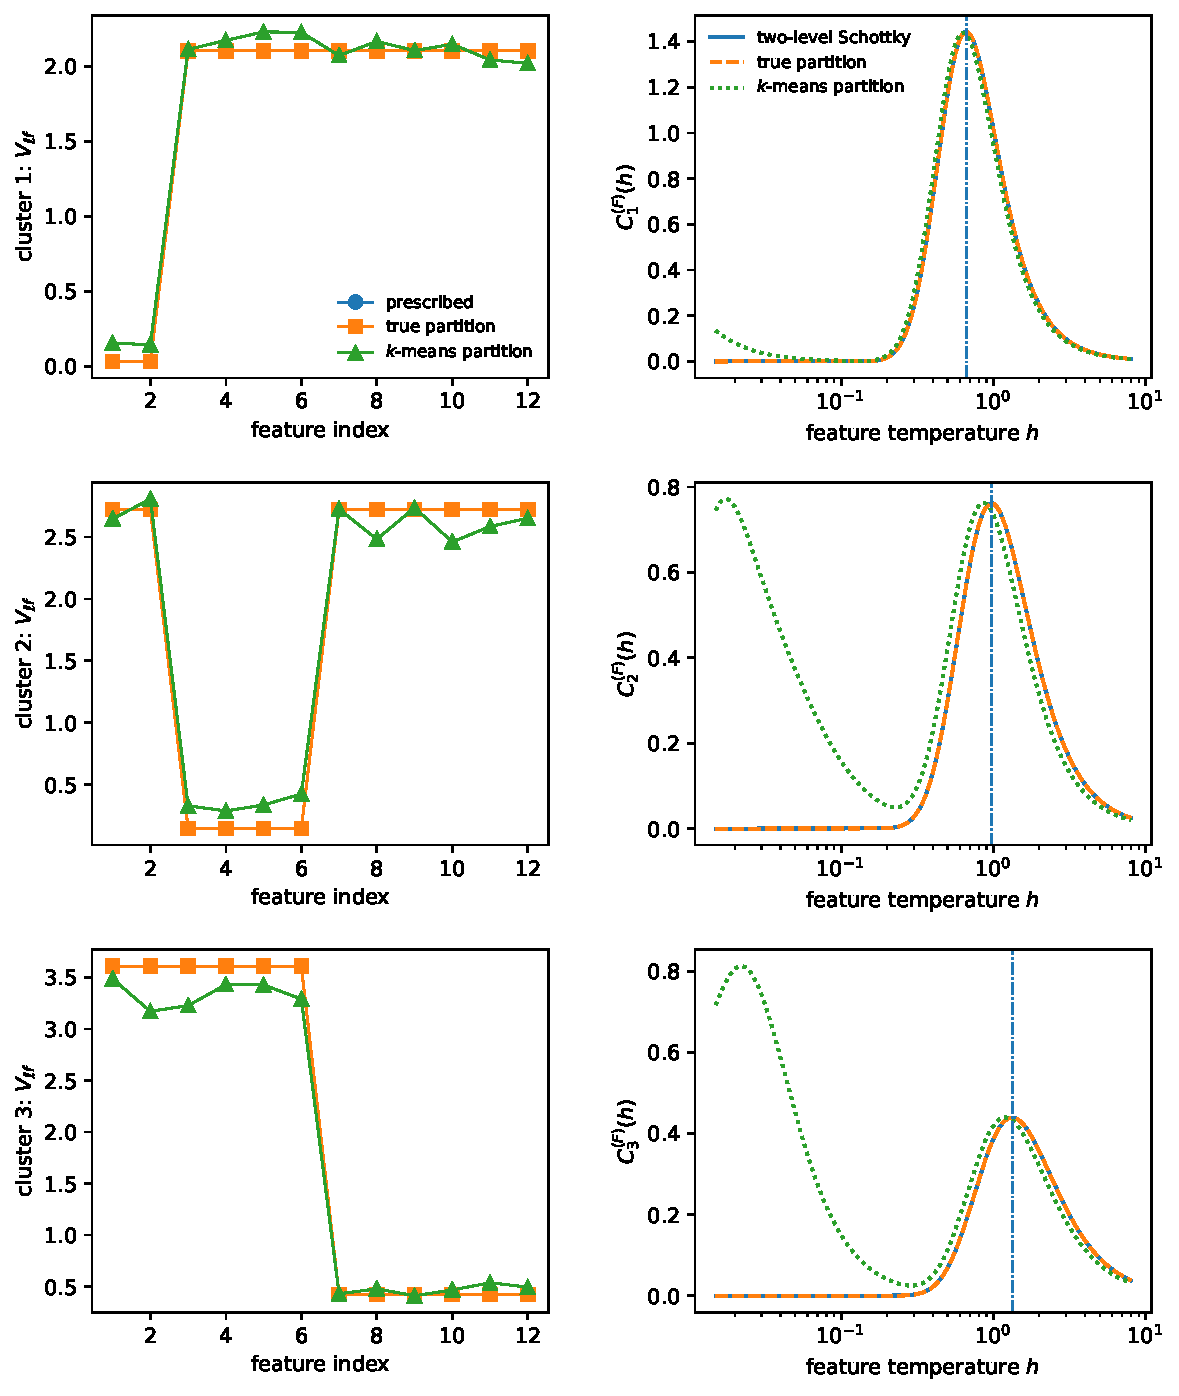
\includegraphics[width=0.94\linewidth]{lac_schottky_validation.pdf}
\caption{Feature-dispersion spectra and response curves for the structured synthetic design. Left: prescribed, true-partition, and aligned initial $k$-means dispersions. Right: the analytic two-level Schottky response, the response from the true partition, and the response from the estimated initial partition. The analytic scale is fixed by the dispersion gap and degeneracy ratio rather than fitted to the numerical response.}
\label{fig:schottky_validation}
\end{figure}


The accuracy experiment is repeated for 30 seeds, 1729 through 1758. For every seed, the same $k$-means initialization is supplied to all LAC variants. The response selector and the supervised oracle are now evaluated on the identical 160-point logarithmic grid over $0.01\le h\le8$, eliminating the asymmetric-grid comparison of the previous analysis. The oracle uses the ground-truth labels only to report the best fixed-$h$ ARI available on this common grid. The \emph{adaptive response rule} recomputes the maximizing global $h$ at every alternating iteration. Because this changes the objective parameter between steps, it is not a fixed-objective descent scheme. We therefore add a \emph{two-pass frozen rule}: $h$ is selected once from the initial $k$-means partition by maximizing the mean cluster response and is then held fixed while the ordinary LAC updates are iterated to a stationary partition. Explicit partition-history tracking detects convergence, cycles of period greater than one, and runs reaching the 100-iteration limit.

Tab.\,\ref{tab:lac_multiseed} reports the results before and after columnwise standardization. On the original synthetic scale, the adaptive and frozen response rules obtain $0.982\pm0.008$ and $0.983\pm0.008$, respectively, compared with $0.988\pm0.006$ for the common-grid oracle. Their paired difference is $-0.0007$ in favor of the frozen rule, with a 95\% bootstrap interval $[-0.0021,0.0006]$, so the interval includes zero and no difference is detected at this sample size. This statement is not an equivalence claim. Relative to the oracle, the frozen rule has a mean deficit of $0.0050$, with bootstrap interval $[-0.0068,-0.0032]$. The adaptive rule improves on fixed $h=1$ by $0.0103$ on average, with interval $[0.0078,0.0127]$.

\begin{table}[htbp]
\centering
\begingroup
\renewcommand{\arraystretch}{1.42}
\setlength{\tabcolsep}{6pt}
\caption{Thirty-realization validation of LAC temperature rules on the structurally heterogeneous synthetic design. Values are mean $\pm$ sample standard deviation of ARI. The same $h$ grid, $0.01\le h\le8$ with 160 logarithmically spaced points, is used by the response selector and oracle. Column standardization is applied globally feature by feature before clustering in the rightmost column.}
\label{tab:lac_multiseed}
\begin{tabular}{lcc}
\toprule
\textbf{Method} & \textbf{Original scale} & \textbf{Standardized features}\\
\midrule
$k$-means initialization & $0.842\pm0.024$ & $0.862\pm0.020$\\
LAC, fixed $h=1$ & $0.972\pm0.010$ & $0.946\pm0.016$\\
LAC, $h=\overline V$ heuristic & $0.957\pm0.015$ & $0.954\pm0.016$\\
LAC, adaptive global response & $0.982\pm0.008$ & $0.977\pm0.009$\\
LAC, two-pass frozen response & $0.983\pm0.008$ & $0.977\pm0.009$\\
LAC, independent clusterwise response & $0.893\pm0.067$ & $0.929\pm0.048$\\
Oracle fixed-$h$ grid & $0.988\pm0.006$ & $0.982\pm0.008$\\
\bottomrule
\end{tabular}
\endgroup
\end{table}

The explicit convergence diagnostic resolves the main theoretical concern raised by the adaptive update. On the original-scale experiment, all 30 adaptive runs and all 30 frozen runs reach a stationary partition; no cycle and no 100-iteration termination is observed. The adaptive rule requires $2.50$ iterations on average, with a maximum of four, and the frozen rule requires $2.33$ iterations on average, also with a maximum of four. Every adaptive run uses exactly two distinct selected temperatures before convergence. These observations do not constitute a convergence theorem for adaptive $h$, but they show that the reported performance is not produced by hidden cycling or truncation. More importantly, the frozen two-pass rule matches the adaptive accuracy while avoiding a changing temperature after the first pass, so the numerical result does not depend on treating the adaptive procedure as a descent algorithm.

The width of the near-optimal region further qualifies the practical value of temperature selection. For each seed we define the connected fixed-$h$ interval containing the oracle maximum and satisfying $\mathrm{ARI}(h)\ge\mathrm{ARI}_{\max}-0.005$. The median multiplicative width of this interval is $1.40$. For the ARI curve averaged over all 30 realizations, the corresponding interval is approximately $0.543\le h\le0.826$, a factor of $1.52$. The median frozen response selection, $h=0.728$, lies about 70\% of the way across this interval on a logarithmic scale and falls inside the seed-specific $0.005$ plateau in 19 of 30 realizations. Thus the problem is neither sharply tuned nor indifferent over an order of magnitude: response selection identifies the correct temperature scale, while the attainable ARI remains moderately tolerant to nearby $h$ values.

The $h=\overline V$ heuristic is informative because it is also covariant under a common global rescaling, yet it performs worse than fixed $h=1$ on the original scale. In the representative construction, the mean variance of irrelevant coordinates exceeds that of relevant coordinates by factors ranging from approximately $8.5$ to $64.9$ across clusters. The arithmetic mean $\overline V$ is therefore dominated by the high-dispersion coordinates. By contrast, the response maximum depends on the contrast and redistribution of occupation probability across the dispersion spectrum rather than only on its absolute mean level. This difference explains why matching the overall dispersion scale is not equivalent to locating the response crossover.

The independent clusterwise rule remains a negative result. Although the fixed-partition weight objective is separable across clusters, cluster-specific temperatures alter subsequent assignments and hence the next spectra. The raw-scale clusterwise rule yields $0.893\pm0.067$, and standardization raises it to $0.929\pm0.048$ without recovering the global rules. The same standardization experiment in Tab.\,\ref{tab:lac_multiseed} shows that all methods move, confirming that the response criterion is covariant under a common global scaling but not invariant under independent feature rescaling.

\begin{figure}[!htbp]
\centering
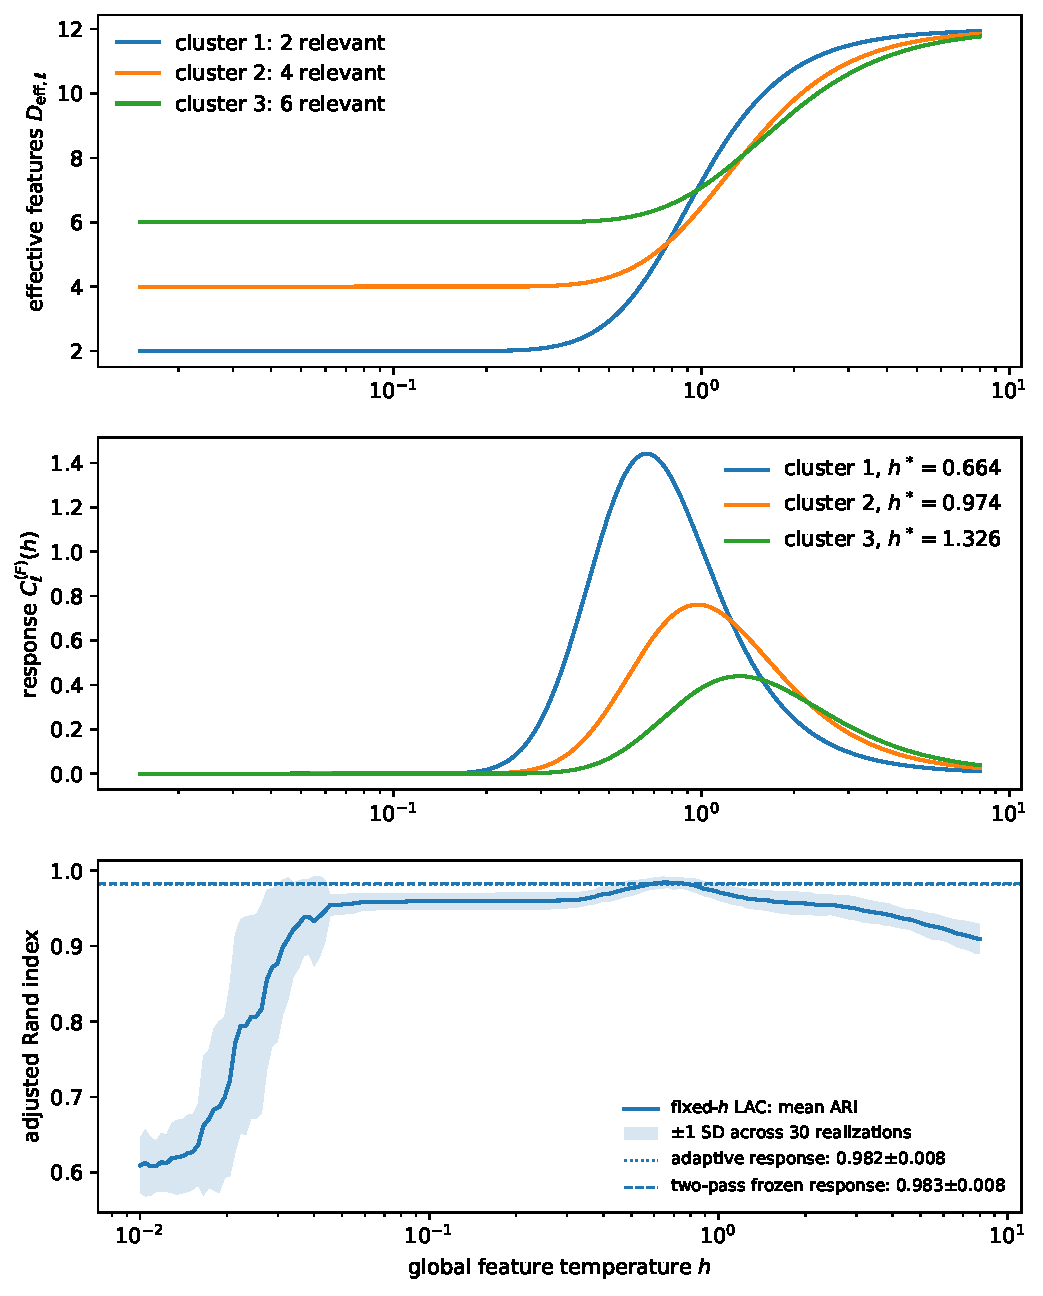
\includegraphics[width=0.86\linewidth]{lac_multiseed_validation.pdf}
\caption{LAC response and multiseed validation. Top: effective feature count for the representative realization, with two, four, and six relevant coordinates. Middle: fixed-spectrum response curves and their separated maxima from Eqs.\,\eqref{eq:representative_hstars:1}--\eqref{eq:representative_hstars:3}. Bottom: mean ARI of fixed-$h$ LAC on the common $h$ grid, with one-standard-deviation band; horizontal lines show the adaptive and two-pass frozen response rules.}
\label{fig:lac_multiseed}
\end{figure}

The synthetic study is complemented by three labeled real datasets distributed with scikit-learn Ref.\,\cite{pedregosa2011scikit}: Iris, Ref.\,\cite{uci_iris}, Wine, Ref.\,\cite{uci_wine}, and Breast Cancer Wisconsin Diagnostic (WDBC), Ref.\,\cite{uci_wdbc}. These datasets contain 150 observations and 4 features, 178 observations and 13 features, and 569 observations and 30 features, respectively. Their features are standardized before clustering, and 30 $k$-means random seeds are used as common initializations. The labels are used only for retrospective ARI evaluation.

\begin{table}[htbp]
\centering
\begingroup
\renewcommand{\arraystretch}{1.38}
\setlength{\tabcolsep}{4.5pt}
\small
\caption{Real-data clustering benchmarks after feature standardization. Values are mean $\pm$ sample standard deviation of ARI over 30 common $k$-means initializations. Zero displayed standard deviation means that the corresponding LAC rule converged to the same partition for all 30 initializations at the reported precision.}
\label{tab:lac_real_benchmarks}
\scriptsize
\begin{tabular}{lcccccc}
\toprule
\textbf{Dataset} & \textbf{$k$-means} & \textbf{$h=1$} & \textbf{$\overline V$} & \textbf{Adaptive} & \textbf{Frozen} & \textbf{Clusterwise}\\
\midrule
Iris & $0.616\pm0.010$ & $0.620\pm0.000$ & $0.716\pm0.000$ & $0.886\pm0.000$ & $0.886\pm0.000$ & $0.886\pm0.000$\\
Wine & $0.897\pm0.000$ & $0.865\pm0.000$ & $0.816\pm0.000$ & $0.847\pm0.000$ & $0.864\pm0.000$ & $0.686\pm0.000$\\
WDBC & $0.663\pm0.009$ & $0.686\pm0.003$ & $0.685\pm0.003$ & $0.712\pm0.000$ & $0.706\pm0.000$ & $0.496\pm0.000$\\
\bottomrule
\end{tabular}
\endgroup
\end{table}

The real-data results are mixed and therefore useful for delimiting the claim. On Iris, both global response rules substantially improve over $k$-means and fixed $h=1$. On Breast Cancer Wisconsin Diagnostic they also improve over those two baselines, although the absolute ARI remains moderate. On Wine, however, $k$-means is best, fixed $h=1$ slightly exceeds the frozen response rule, and the adaptive response rule is lower still. The response criterion should therefore be regarded as a data-dependent temperature diagnostic rather than as a universally superior clustering rule. The absence of a universal win is consistent with the intended scope of the paper and prevents the controlled synthetic result from being generalized beyond its evidence.

\subsubsection{Matched-grid unsupervised temperature-selection baselines}
\label{subsubsec:h_baselines}

The response rule is also compared with two genuinely unsupervised selectors rather than only with fixed numerical choices of $h$. Average silhouette width, Ref.\,\cite{rousseeuw1987silhouette}, is evaluated on the Euclidean geometry of the data for each candidate fixed-$h$ partition. A perturbation-stability score, following the general stability principle of Ben-Hur, Elisseeff, and Guyon, Ref.\,\cite{benhur2002stability}, is computed from pairwise ARI among four small-noise perturbations of the same dataset. To keep the computational comparison matched, response, silhouette, stability, and retrospective oracle selection use the same 36-point logarithmic grid $0.02\le h\le6$. The synthetic comparison uses ten seeds and each real dataset uses five common seeds; these runs are separate from the 30-seed estimates in Tabs.\,\ref{tab:lac_multiseed} and \ref{tab:lac_real_benchmarks}.

\begin{table}[htbp]
\centering
\small
\caption{Matched-grid comparison of temperature selectors. Values are mean $\pm$ sample standard deviation of retrospective ARI. Response, silhouette, and stability are unsupervised; the oracle uses labels only to show the best fixed-$h$ value on the same grid.}
\label{tab:h_selector_baselines}
\begin{tabular}{lccccc}
\toprule
\textbf{Dataset} & \textbf{$k$-means} & \textbf{Response} & \textbf{Silhouette} & \textbf{Stability} & \textbf{Oracle}\\
\midrule
Synthetic & $0.840\pm0.032$ & $0.982\pm0.009$ & $0.916\pm0.019$ & $0.971\pm0.011$ & $0.985\pm0.006$\\
Iris & $0.615\pm0.012$ & $0.886\pm0.000$ & $0.615\pm0.012$ & $0.886\pm0.000$ & $0.886\pm0.000$\\
Wine & $0.897\pm0.000$ & $0.864\pm0.000$ & $0.897\pm0.000$ & $0.894\pm0.007$ & $0.898\pm0.000$\\
WDBC & $0.667\pm0.008$ & $0.712\pm0.000$ & $0.682\pm0.000$ & $0.693\pm0.039$ & $0.724\pm0.000$\\
\bottomrule
\end{tabular}
\end{table}

\begin{figure}[!htbp]
\centering
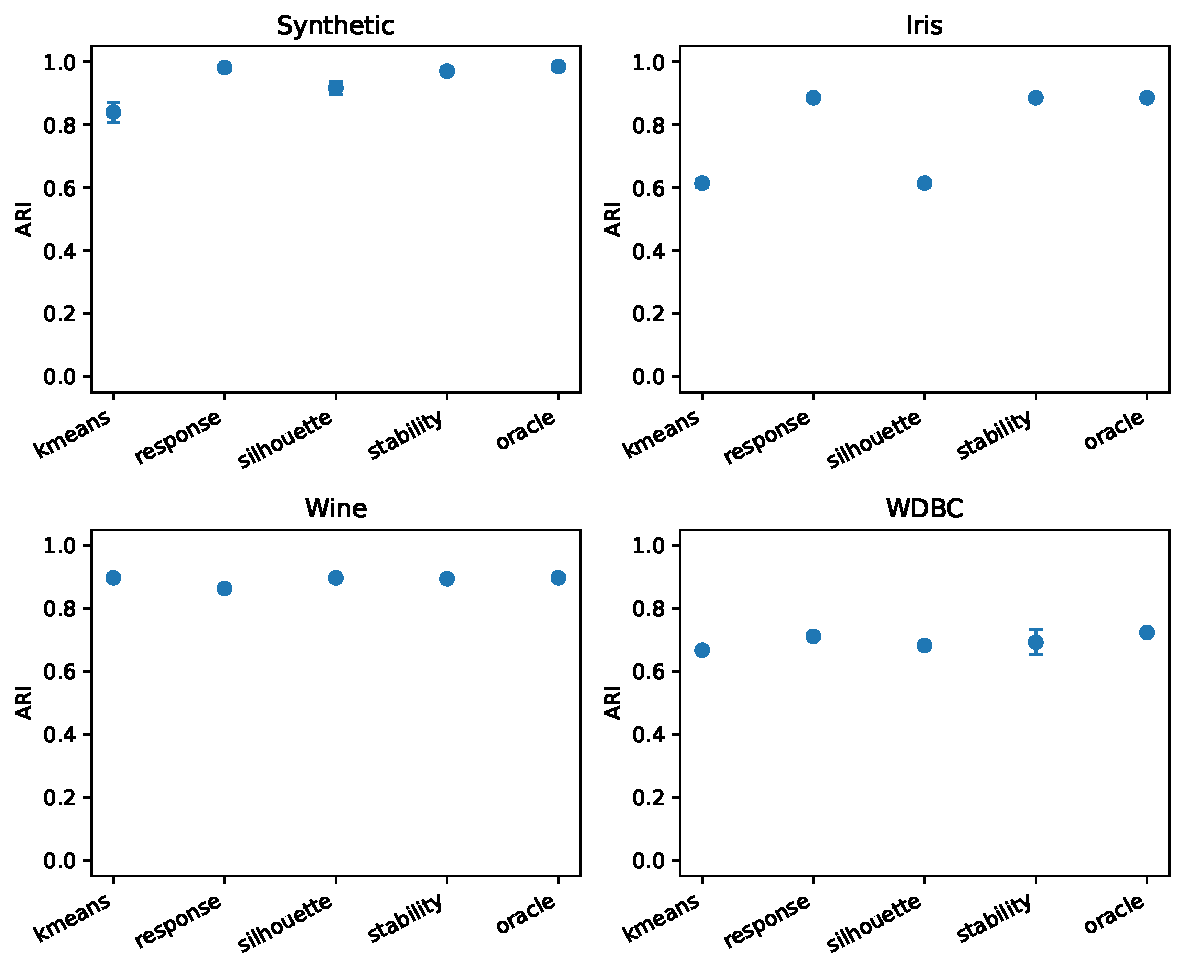
\includegraphics[width=0.90\linewidth]{lac_selector_baselines.pdf}
\caption{Matched-grid comparison of unsupervised temperature selectors. Error bars show sample standard deviations across the dedicated baseline runs. The oracle is retrospective and is included only as a reference scale.}
\label{fig:h_selector_baselines}
\end{figure}


\subsubsection{Controlled robustness beyond the reference generator}
\label{subsubsec:lac_stress}

A one-factor-at-a-time stress study tests limitations that are not represented by changing the random seed alone. Eight seeds are evaluated per setting while varying center separation, cluster-size imbalance, the number of dimensions through additional irrelevant coordinates, and planar rotations that mix coordinates that are relevant for one cluster with coordinates that are irrelevant for another. Fig.\,\ref{fig:lac_stress} reports $k$-means, fixed $h=1$, and the two-pass global response rule. On the unmodified reference setting the response ARI is approximately 0.980. Reducing the center factor to $0.5$ changes it to 0.653; a four-to-one cluster-size ratio gives 0.978; increasing the ambient dimension to 96 gives 0.965; and a $45^\circ$ rotation gives 0.071. The rotation experiment is especially diagnostic because it directly attacks the axis-aligned local-feature assumption: any deterioration there is a structural limitation of diagonal feature weighting rather than a failure of numerical temperature optimization.

\begin{figure}[!htbp]
\centering
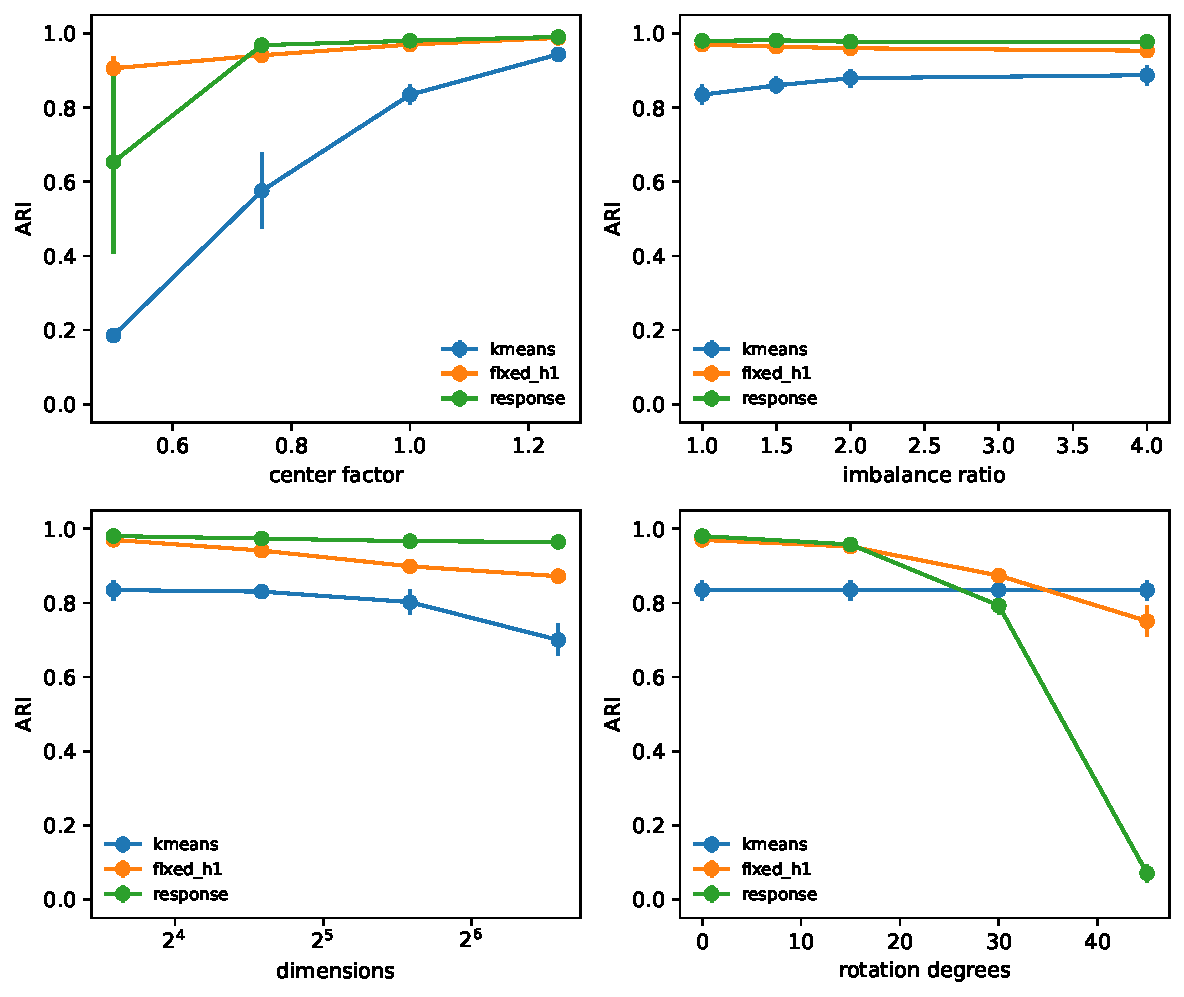
\includegraphics[width=0.92\linewidth]{lac_stress_tests.pdf}
\caption{Controlled LAC stress tests. One factor is varied at a time around the reference synthetic generator: center separation, cluster-size imbalance, added irrelevant dimensions, and rotation away from axis-aligned feature relevance. Curves show mean ARI across eight seeds with one-sample-standard-deviation error bars.}
\label{fig:lac_stress}
\end{figure}


\subsection{Assignment bifurcation versus finite feature crossover}
\label{subsec:annealing_demo}

The same representative synthetic dataset is used for a deterministic-annealing control. Three codevectors are initialized at the global mean and optimized while the assignment temperature is decreased geometrically. For squared Euclidean distortion, the first loss of stability of the coincident solution occurs at the deterministic-annealing critical scale associated with the largest covariance eigenvalue, as developed by Rose, Gurewitz, and Fox Ref.\,\cite{rose1990phase}. In the present dataset the predicted value is $T_c=12.501$, while the first numerically resolved separation of the codevectors occurs at $T=12.360$ on the finite temperature grid.

Fig.\,\ref{fig:annealing_bifurcation} plots the codevector-separation order parameter alone; the LAC response curves are not repeated because they already appear in Fig.\,\ref{fig:lac_multiseed}. The contrast is therefore direct without duplicating a panel: deterministic annealing changes the optimized representation and displays a bifurcation, whereas each fixed LAC dispersion spectrum gives an analytic finite-system crossover. This distinction is also consistent with the broader statistical-physics clustering literature, including the Potts-spin construction of Blatt, Wiseman, and Domany Ref.\,\cite{blatt1996spc}, where clustering structure is associated with collective thermodynamic organization rather than with a finite independent feature spectrum.

\begin{figure}[!htbp]
\centering
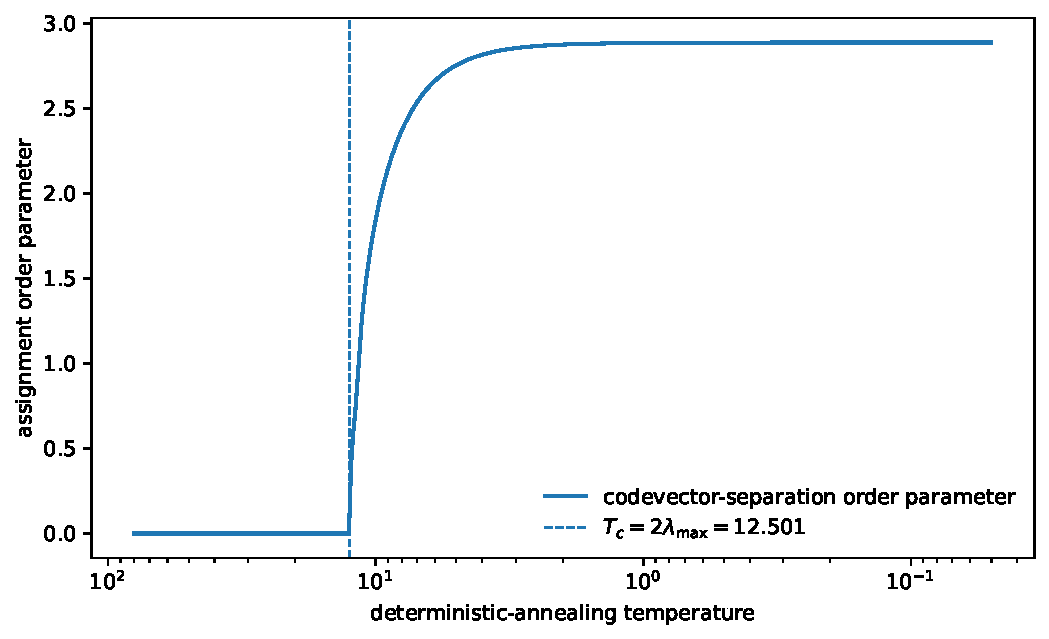
\includegraphics[width=0.80\linewidth]{annealing_bifurcation.pdf}
\caption{Deterministic-annealing control on the representative synthetic dataset. The order parameter measures root-mean-square separation of the three optimized codevectors. The dashed line is the theoretical first critical temperature $T_c=2\lambda_{\max}=12.501$; the first resolved split on the numerical schedule occurs at $12.360$.}
\label{fig:annealing_bifurcation}
\end{figure}

\subsection{Self-similar SNE scaling, errors in variables, and the Wine deviation}
\label{subsec:sne_scaling}

For a fixed anchor, multiplying every neighbor distance by a common factor $\lambda$ multiplies the quadratic energy spectrum by $\lambda^2$. The canonical probabilities and their entropy remain unchanged if the local temperature is transformed by the same factor:
\begin{equation}
    E_{ij}^{(N)}\mapsto\lambda^2E_{ij}^{(N)}
    \quad\Longrightarrow\quad
    T_i^{(N)}\mapsto\lambda^2T_i^{(N)}.
    \label{eq:sne_similarity_scaling}
\end{equation}
For a reciprocal-length density proxy $\rho\mapsto\lambda^{-1}\rho$, Eq.\,\eqref{eq:sne_similarity_scaling} predicts
\begin{equation}
    \frac{\mathrm{d}\ln\left(T_i^{(N)}\right)}{\mathrm{d}\ln\left(\rho_i\right)}=-2.
    \label{eq:sne_density_slope_prediction}
\end{equation}
The top panel of Fig.\,\ref{fig:sne_density_scaling} is an exact self-similar control: one uniform sample of 240 points in five dimensions is rescaled by six factors between $0.6$ and $2.2$. At perplexity 20 the recovered median-temperature slope is $-2.000$ to numerical precision.

The middle panel isolates regression dilution. Equal-variance Gaussian noise is added to both logarithmic coordinates of the exact control, so the equal-error assumption of ordinary total least squares (TLS) is satisfied by construction. Ordinary least squares (OLS) attenuates the slope to $-1.716$, whereas TLS recovers $-2.016$. This control does not justify the equal-error assumption for Wine; it only demonstrates the direction of the bias under a case where the TLS assumption is known to hold.

The lower panel uses the standardized Wine Recognition dataset, Ref.\,\cite{uci_wine}. The SNE temperature is solved independently for all 178 observations at perplexity 20, and the ten-neighbor reciprocal-distance proxy is
\begin{equation}
    \rho_i^{(10)}
    :=\left[
    \frac{1}{10}
    \sum_{j\in\mathcal N_i^{(10)}}\|x_i-x_j\|_2
    \right]^{-1}.
    \label{eq:density_proxy}
\end{equation}
The Spearman effect size is $\rho_S=-0.643$ with asymptotic two-sided $p=3.87\times10^{-22}$. OLS gives slope $-1.123$ with a 95\% bootstrap interval $[-1.272,-0.951]$. Under the unverified equal-error assumption, TLS gives $-1.859$ with bootstrap interval $[-2.227,-1.611]$. Changing the density proxy from 10 to 20 and 30 neighbors moves the OLS slopes to $-1.325$ and $-1.456$ and the TLS slopes to $-1.906$ and $-1.969$, respectively. The discrepancy from $-2$ is therefore consistent with a combination of proxy mismatch and regression dilution, but the Wine calculation alone cannot identify their relative contributions; anisotropy, boundary effects, and the small sample in 13 standardized dimensions remain additional sources of deviation.

\begin{figure}[!htbp]
\centering
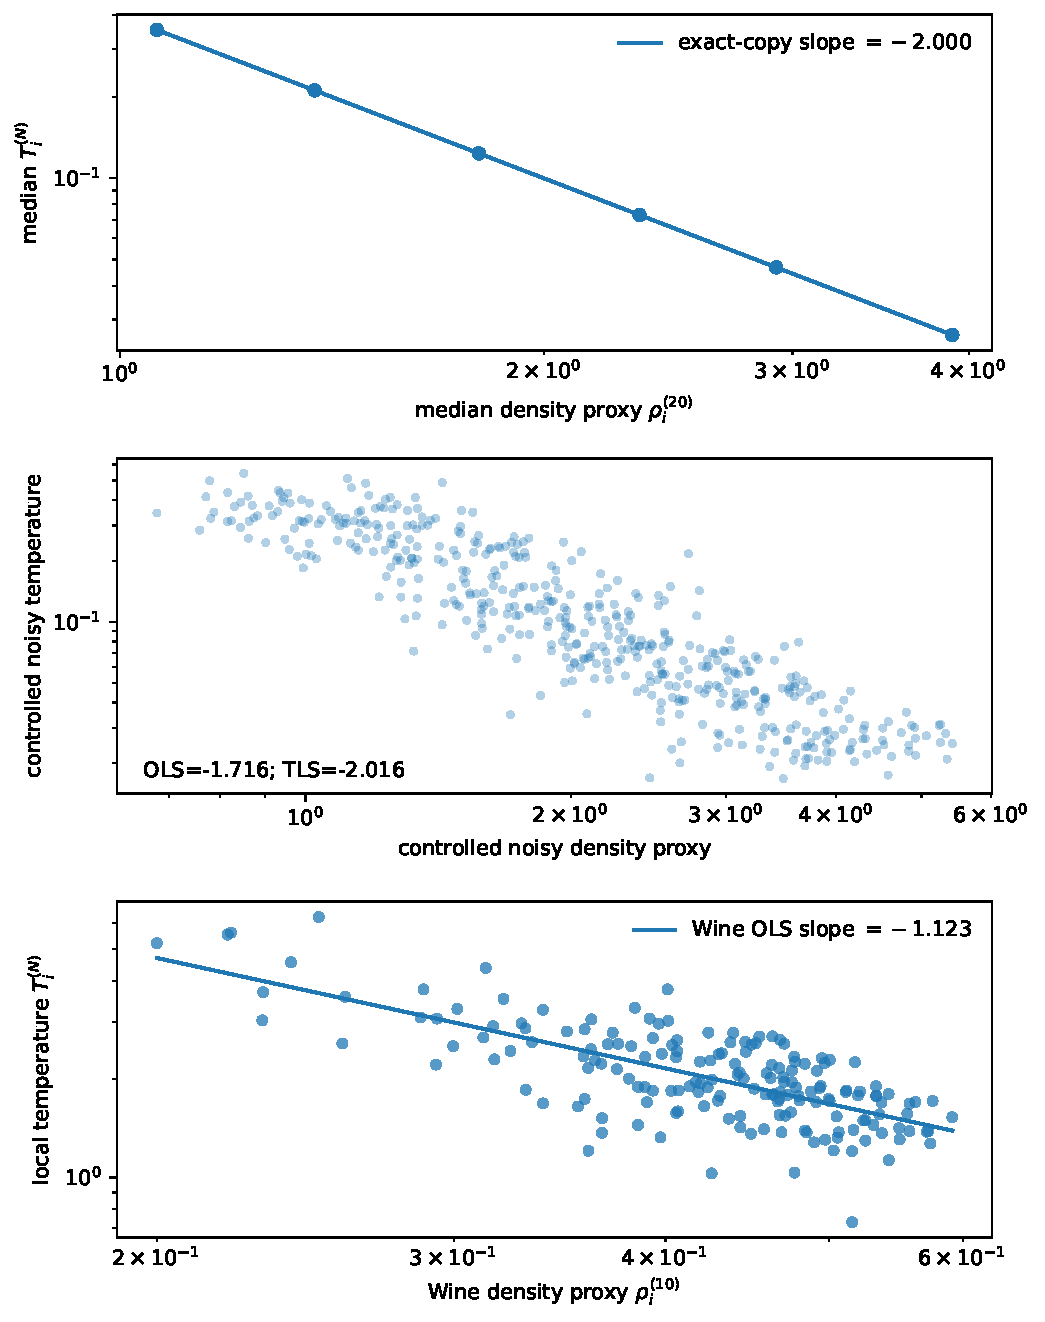
\includegraphics[width=0.86\linewidth]{sne_density_scaling.pdf}
\caption{Fixed-perplexity SNE scaling. Top: exact rescaled-copy control recovering the predicted slope $-2$. Middle: controlled equal-variance noise in both logarithmic variables, for which OLS attenuates the slope while TLS recovers the known value. Bottom: standardized Wine data, where OLS gives $-1.123$ and TLS gives $-1.859$ under its additional error-ratio assumption.}
\label{fig:sne_density_scaling}
\end{figure}

\subsection{Neighbor response as a bandwidth-tolerance diagnostic}
\label{subsec:numerical_response}

The Wine response distribution has a direct numerical interpretation through Corollary\,\ref{cor:perplexity_tolerance}. Its median and 95th percentile are
\begin{subequations}
\label{eq:wine_response_summary}
\begin{empheq}[left=\empheqlbrace]{align}
    \operatorname{median}_i C_i^{(N)}&=1.447,\label{eq:wine_response_median}\\
    Q_{0.95}\!\left(C_i^{(N)}\right)&=2.605.\label{eq:wine_response_q95}
\end{empheq}
\end{subequations}
For a 1\% target relative perplexity error, Eq.\,\eqref{eq:perplexity_sigma_tolerance} therefore requires approximately $0.346\%$ relative bandwidth accuracy at the median anchor and $0.192\%$ at the 95th percentile. These values are not a new entropy identity; they are an operational consequence that can be used to set an anchor-specific stopping tolerance in a bandwidth solver. The derivative itself is related to the entropic-affinity root-finding analysis of Vladymyrov and Carreira-Perpi\~n\'an Ref.\,\cite{vladymyrov2013entropic}; the reported distribution and tolerance conversion are the quantities evaluated here.

\begin{figure}[!htbp]
\centering
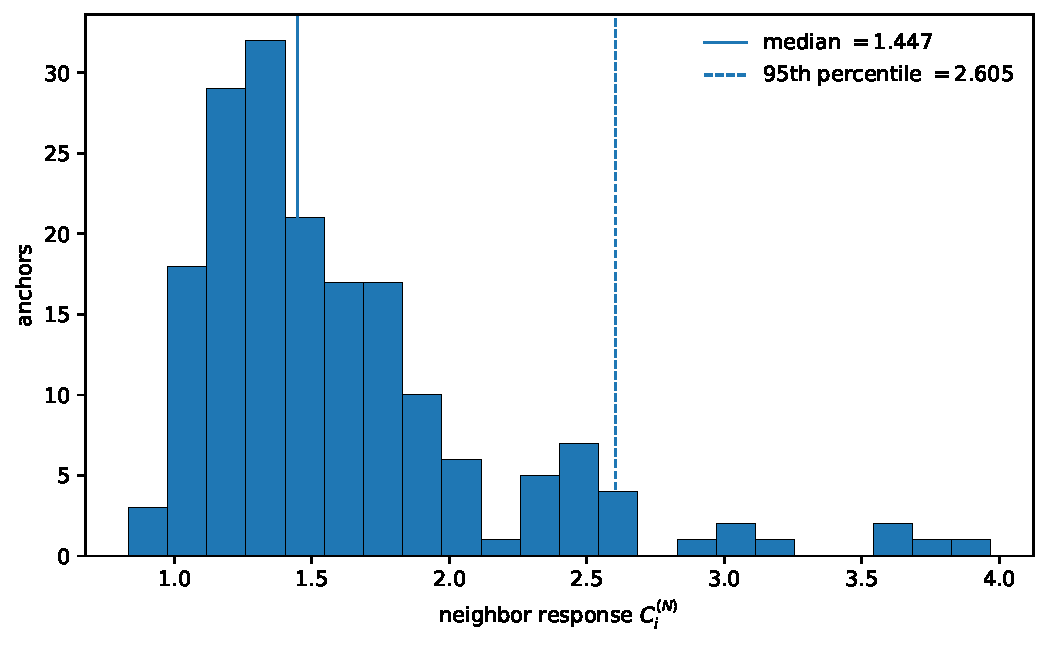
\includegraphics[width=0.80\linewidth]{sne_neighbor_response.pdf}
\caption{Distribution of the local SNE response $C_i^{(N)}$ on the standardized Wine dataset at perplexity 20. The response determines the first-order bandwidth accuracy required to enforce a prescribed local perplexity tolerance through Eq.\,\eqref{eq:perplexity_sigma_tolerance}.}
\label{fig:sne_neighbor_response}
\end{figure}

The numerical evidence therefore supports a narrower but stronger conclusion than the earlier single-seed analysis. A global LAC response rule is consistently close to the oracle temperature on the controlled design and improves over several unsupervised baselines, whereas the naive clusterwise response rule fails. Deterministic annealing displays the expected bifurcation on the same geometry. In SNE, the response yields a directly usable bandwidth tolerance, and the density-scaling experiments distinguish the exact self-similar law from regression and geometric effects that are present in real data.

\FloatBarrier

\section{Limitations and reproducibility}
\label{sec:limitations}

The original 30-seed synthetic experiment varies random realization while holding the structural design fixed. The added one-factor stress tests extend this evidence to changes in overlap, imbalance, dimensionality, and rotation, but they still do not constitute a broad benchmark suite: the clusters remain Gaussian and the response study remains centered on diagonal LAC feature weighting. The rotation experiment is particularly relevant because it exposes the expected limitation of axis-aligned relevance. The real-data benchmarks likewise remain small in number. Broader datasets and non-Gaussian geometries are therefore still required before the response criterion can be treated as a general model-selection procedure.

The adaptive global rule changes $h$ between alternating iterations and consequently does not minimize one fixed objective throughout its trajectory. Explicit history tracking found no cycles or iteration-limit terminations in the 30 synthetic runs, but this empirical observation is not a convergence proof. The two-pass frozen rule was introduced precisely to separate temperature selection from subsequent fixed-$h$ optimization. Its paired bootstrap interval relative to the adaptive rule includes zero on the controlled design, so no difference is detected at this sample size; this is not treated as evidence of formal equivalence. The frozen rule nevertheless avoids repeated changes of the objective parameter. The negative clusterwise result remains stronger: separability of the fixed-partition feature-weight problem does not imply that independent cluster temperatures are stable under reassignment.

Phase-transition language requires a distinct caution. The fixed feature spectrum has an analytic partition function for every $h>0$, so the maxima of Eq.\,\eqref{eq:lac_response} are finite-system crossovers. Deterministic annealing and superparamagnetic clustering, Refs.\,\cite{rose1990phase,blatt1996spc,wiseman1998spc}, involve optimized or interacting representations in which collective organization can change qualitatively. The present comparison separates these mechanisms; it does not reinterpret the LAC crossover as a thermodynamic phase transition.

The SNE scaling experiment isolates only part of the deviation observed on Wine. The exact $-2$ law follows under global self-similar rescaling, and the controlled errors-in-variables experiment shows how OLS attenuation and TLS correction behave when equal log-scale error variances are imposed by construction. In the Wine data that equality is unknown. TLS is therefore a sensitivity analysis rather than a privileged estimator, while density-proxy mismatch, anisotropy, boundaries, and finite sample size remain confounded.

The dual feature--neighbor construction in Sec.\,\ref{sec:dual} is prospective. It defines how a feature ensemble could modify the neighbor energy, but no monotone-descent theorem, complexity bound, consistency result, or embedding benchmark is supplied. Its inclusion exposes a mathematically natural next problem rather than a completed method.

\FloatBarrier

\section{Conclusion}
\label{sec:conclusion}

The useful content of the statistical-mechanical comparison appears only after normalized-exponential identities are separated from algorithm-specific state variables and measurable response. Deterministic annealing, superparamagnetic clustering, softmax normalization, energy-based learning, and entropic affinities already establish much of the mathematical vocabulary. The distinction developed here is narrower: LAC distributes probability over feature states in its weight subproblem, SNE distributes probability over candidate neighbors, and deterministic annealing distributes probability over assignments or codevectors.

That distinction leads to a specific spectral mechanism. For a two-level LAC dispersion spectrum, the response is a finite Schottky anomaly whose peak is fixed by the dispersion gap and the degeneracy ratio. The synthetic experiment confirms the analytic peak on the true partition and quantifies its displacement when the spectrum is estimated from the initial $k$-means partition. Broad or rotated spectra provide corresponding failure modes rather than unexplained exceptions.

That distinction leads to a specific spectral mechanism. For a two-level LAC dispersion spectrum, the response is a finite Schottky anomaly whose peak is fixed by the dispersion gap and the degeneracy ratio. The synthetic experiment confirms the analytic peak on the true partition and quantifies its displacement when the spectrum is estimated from the initial $k$-means partition. Broad or rotated spectra provide corresponding failure modes rather than unexplained exceptions.

That distinction leads to a specific spectral mechanism. For a two-level LAC dispersion spectrum, the response is a finite Schottky anomaly whose peak is fixed by the dispersion gap and the degeneracy ratio. The synthetic experiment confirms the analytic peak on the true partition and quantifies its displacement when the spectrum is estimated from the initial $k$-means partition. Broad or rotated spectra provide corresponding failure modes rather than unexplained exceptions.

That distinction leads to testable consequences. Across 30 realizations of one controlled heterogeneous design, both global response rules remain close to the retrospectively optimal fixed temperature. The two-pass frozen rule performs at least as well as the adaptive rule within the observed uncertainty while avoiding repeated changes of the objective parameter. The experiment also supplies two qualifications. First, the near-optimal ARI region has a finite but non-negligible width, so temperature selection is useful without being sharply tuned. Second, independently maximizing one response per cluster degrades performance, showing that fixed-partition separability does not transfer automatically to the full alternating dynamics. The three real benchmarks reinforce the same caution: response selection improves clustering on Iris and Breast Cancer Wisconsin Diagnostic but does not improve on $k$-means for Wine.

For SNE, the response has a direct numerical use rather than only a thermodynamic interpretation. It converts a target perplexity accuracy into an anchor-specific first-order bandwidth tolerance, and direct perturbation experiments across four perplexities show where that linearization is quantitatively accurate. The result is explicitly conditional on a chosen perplexity and is complementary to multiscale, perplexity-free, and automatic-perplexity methods rather than a replacement for them. Controlled scaling experiments remain a consistency check that separates the exact self-similar law from regression and geometric effects present in Wine. The generalized Student discussion is deliberately limited to a conditional quadratic-energy representation and is not treated as an independent empirical result.

The resulting picture is more limited but more defensible than a generic Gibbs reinterpretation. Response functions can be reported as algorithmic diagnostics, tested against clustering accuracy and numerical tolerances, and rejected when their naive extension fails. Broader clustering benchmarks and a separately validated feature--neighbor embedding remain the next substantive steps.

\section*{Data and code availability}
All numerical figures, CSV summaries, random seeds, and experiment drivers used in Sec.\,\ref{sec:numerical} are versioned with the manuscript under \path{paper/experiments/}. The executable driver \path{paper/experiments/run_experiments.py} regenerates the tabular outputs in \path{paper/experiments/assets/}, the companion raster figure exports in \path{paper/experiments/assets/source_images/}, and the PDF figures consumed directly by the LaTeX source in \path{paper/figures/}. File names are stable and each workflow execution overwrites the current derived artifacts; historical versions are retained by Git. The fully pinned execution environment is listed in \path{requirements.lock}, and the three real datasets are loaded from scikit-learn without a network request at execution time Ref.\,\cite{pedregosa2011scikit}.

\section*{Artificial intelligence use disclosure}
GPT-5.6 Sol (OpenAI, used during the August 2026 revision) was used to assist with implementation and review of repository software code, software tests, and preparation of the BibTeX bibliography file. Claude Opus was used as an auxiliary tool for technical discussion of the subject matter, critical review of the manuscript, bibliographic research, auxiliary checking of mathematical passages, and checks of textual coherence; all such checks were independently reviewed by the author. Grammarly was used for grammatical review. All mathematical claims, interpretations, references, code, numerical results, and final manuscript content were reviewed by the author, who retains full responsibility for the published work.


\printbibliography

\end{document}
